% details-of-test-conditions.tex

\textcolor{red}{
	\chapter{Thermal Analysis}
}
%\textcolor{red}{XXX note: layers might be at different temps, tested temps may not be exceeded.}


The thermal protection of a hypersonic launch vehicle is essential to its operation, and is one of the most significant challenges that must be overcome before airbreathing launch systems can become a reality. The SPARTAN-based launch system in this study includes nearly the same thermal protection that is used in previous SPARTAN studies, that has been assumed to be able to protect the SPARTAN throughout its launch trajectory\cite{Preller2018a}. However, no detailed thermal analysis of the SPARTAN has been carried out to date. This section aims to analyse the thermal protection system of the SPARTAN, in order to determine whether it is sufficient for operation to a first approximation. While the purpose of this work is not to significantly redesign a launch vehicle, the design of the SPARTAN's TPS is investigated to analyse the level of thermal protection that may be necessary for future operation. 


%\textcolor{red}{XXX I dont know how to express why reynolds analogy is not valid.. is it just radiating shock layer effects? Then why would it be specific to a part of the leading edge that isnt near the shock?}

During launch, the launch system is exposed to large aerothermal loading that must be resisted using passive thermal protection systems. The heat flux over the trajectory is modelled at various locations on the SPARTAN and third stage, and integrated over the trajectory using 1-D heat conduction analysis to determine the efficacy of the thermal protection system. For the body, the criteria for thermal protection system effectiveness is that the temperature at the internal surface of the thermal protection system does not melt or cause failure in the internal structure. For the nose tips and the wing leading edges it is assumed that the thermal protection system will not be directly attached to the internal insulation and will have their own isolated structure, so that the criteria for thermal protection system success is that the temperature at these points is maintained within the operable limits of the external thermal protection system materials. 

The heat transfer coefficients on the body of the vehicle are computed using Reynolds analogy: 
\begin{equation}
c_h = \frac{c_f}{2s},
\end{equation}
where $c_f$ is the coefficient of friction and $s$ is the Reynold's analogy factor, assumed to be 1.16\cite{Ward2018}. 
This solution is performed within the viscous solver VC3D, at specific locations around the body of the scramjet accelerator and third stage, as shown in Figure \ref{fig:Q_pos}. On the scramjet accelerator, the nose stagnation point (\textcolor{red}{1}) and wing leading edges (\textcolor{red}{2}) are examined, along with a point midway along the nose (\textcolor{red}{3}), as well as midway along the cowl front (\textcolor{red}{4}), one-quarter of the length along the wing (\textcolor{red}{5}), and on the tip of the tail (\textcolor{red}{6}) on the windward side. On the third stage, the stagnation point on the nose (\textcolor{red}{1}) is examined, along with a point half way along the nose cone (\textcolor{red}{2}), and a point half way along the cylindrical cowl (\textcolor{red}{3}) on the windward side. These points are judged to be locations of potential high heat loads on the vehicles, and are examined as worst-case examples for thermal analysis. 

\begin{figure}[!ht]
	
\begin{subfigure}{.5\textwidth}
	\centering
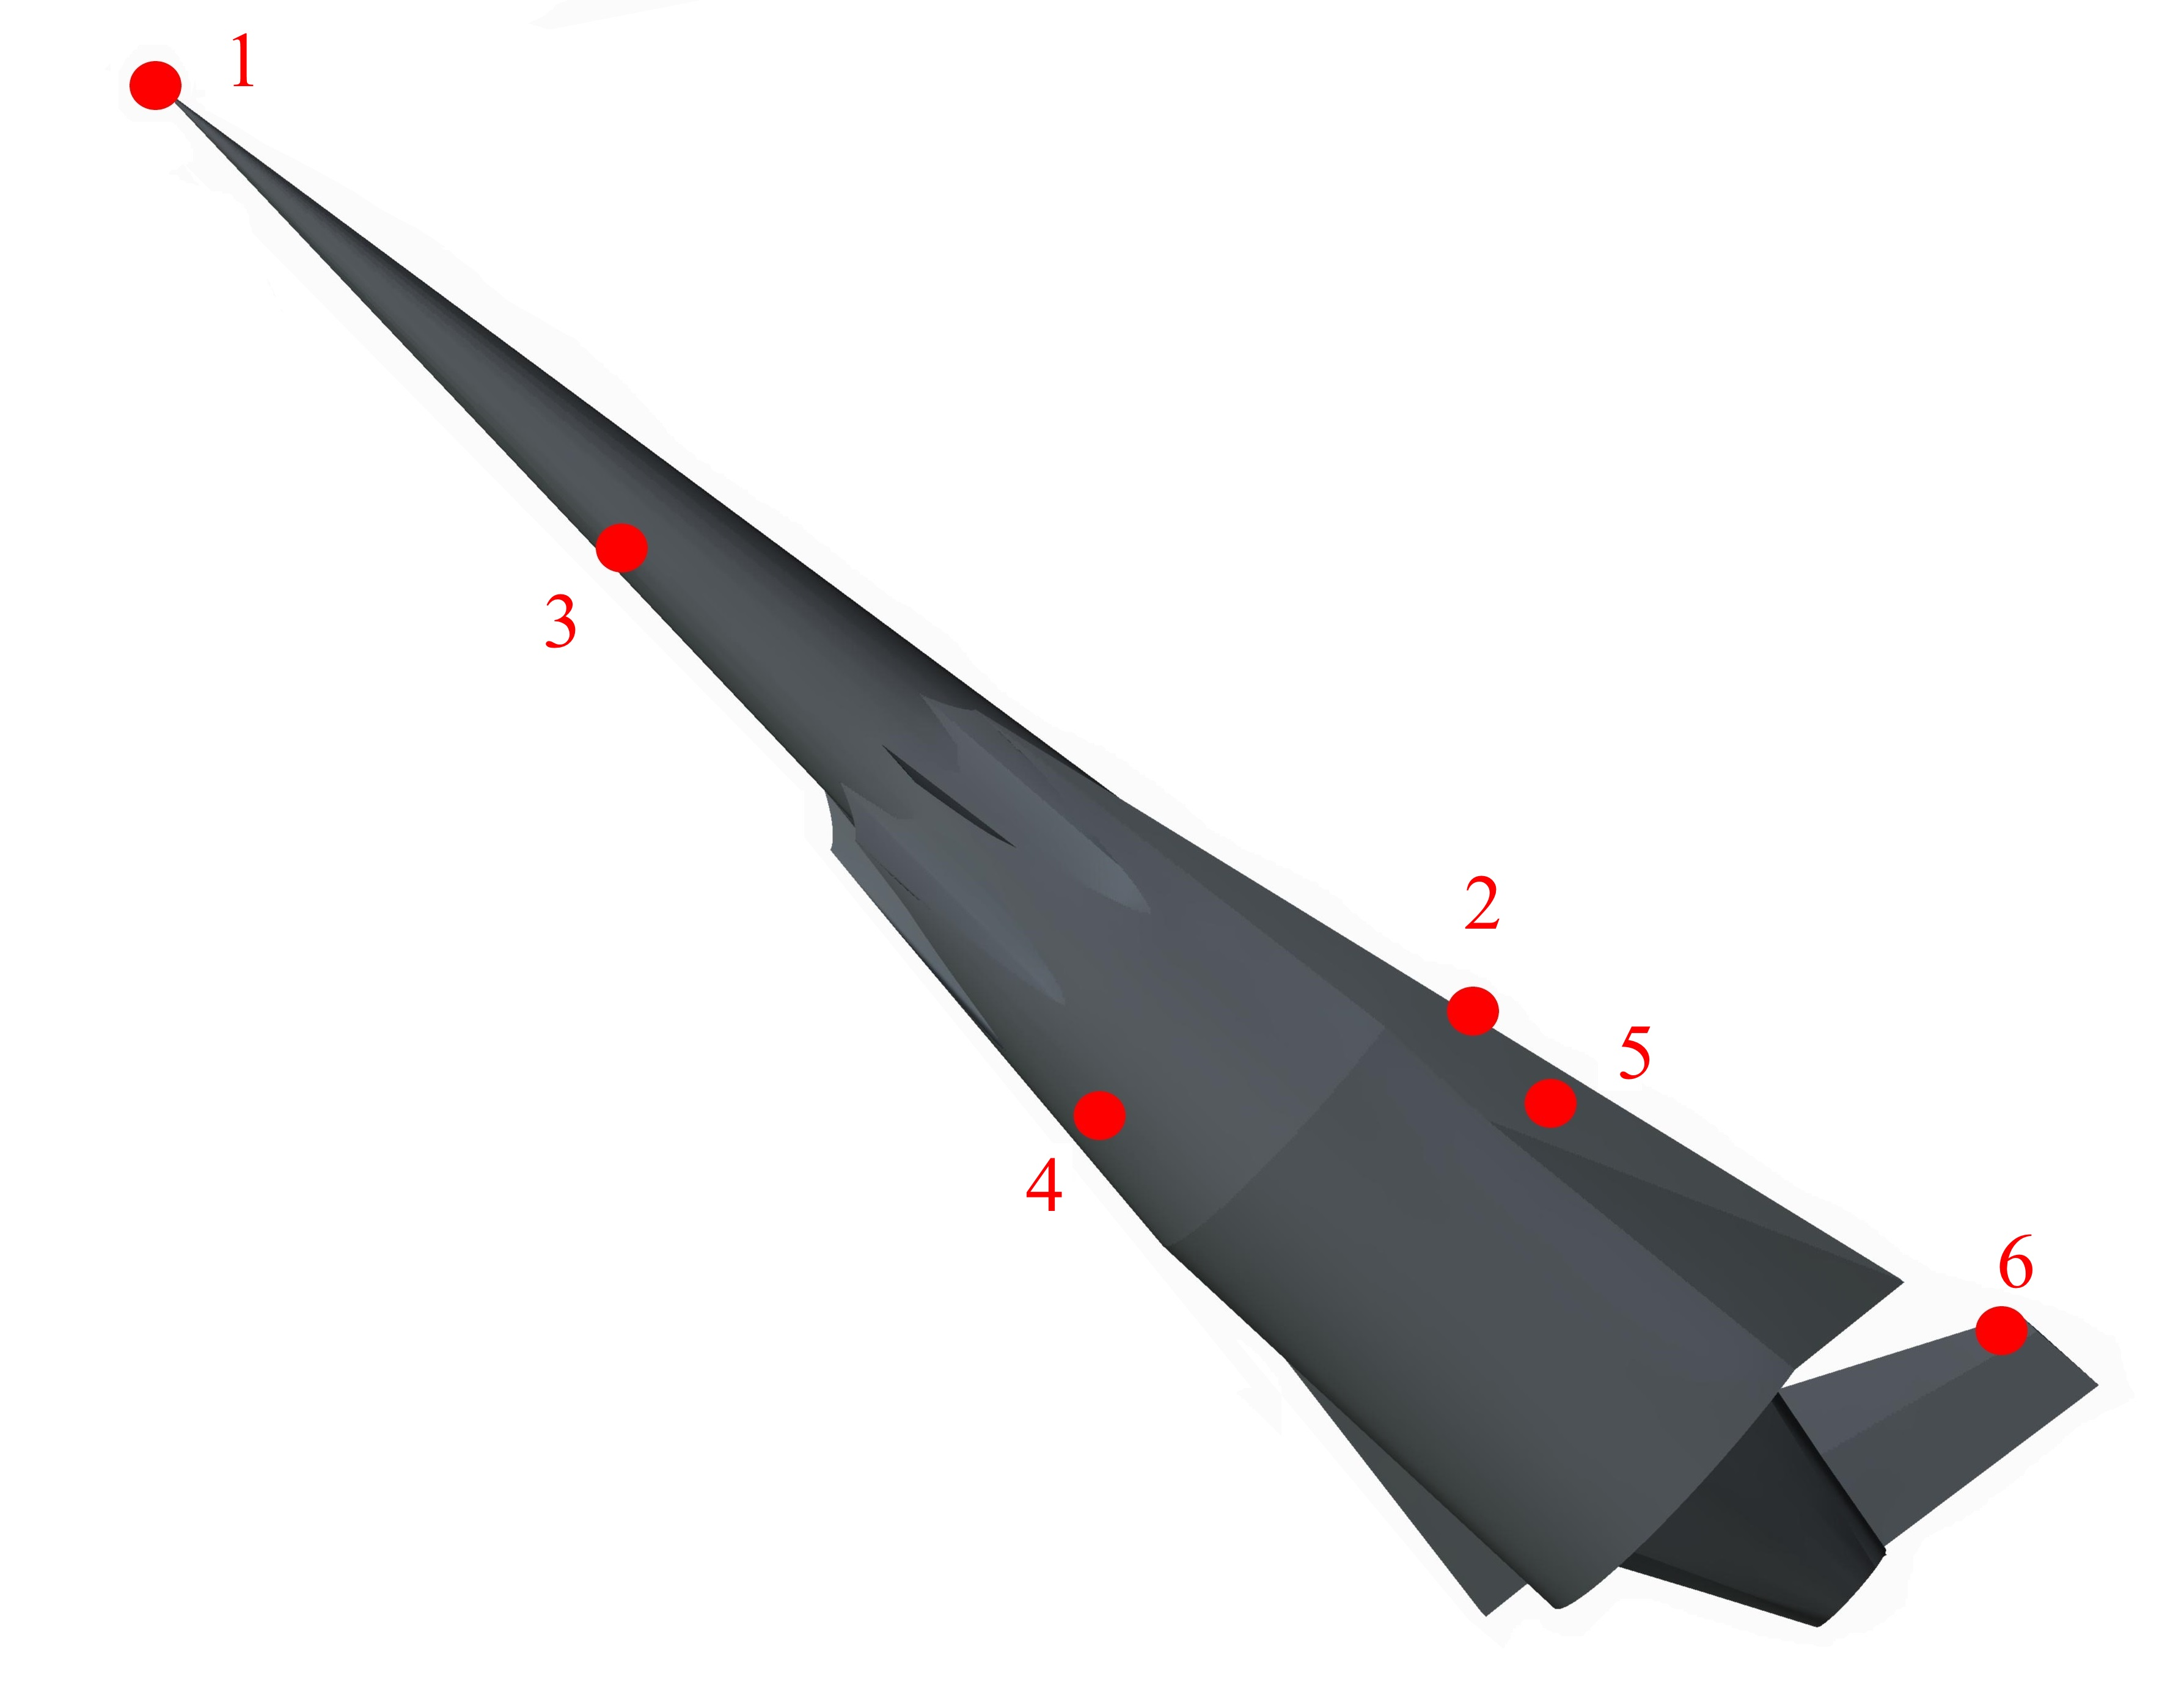
\includegraphics[width=0.9\linewidth]{figures/A1_uncertainty-analysis/Q_pos}
\caption{The points examined on the scramjet accelerator.}
\end{subfigure}
\begin{subfigure}{.5\textwidth}
	\centering
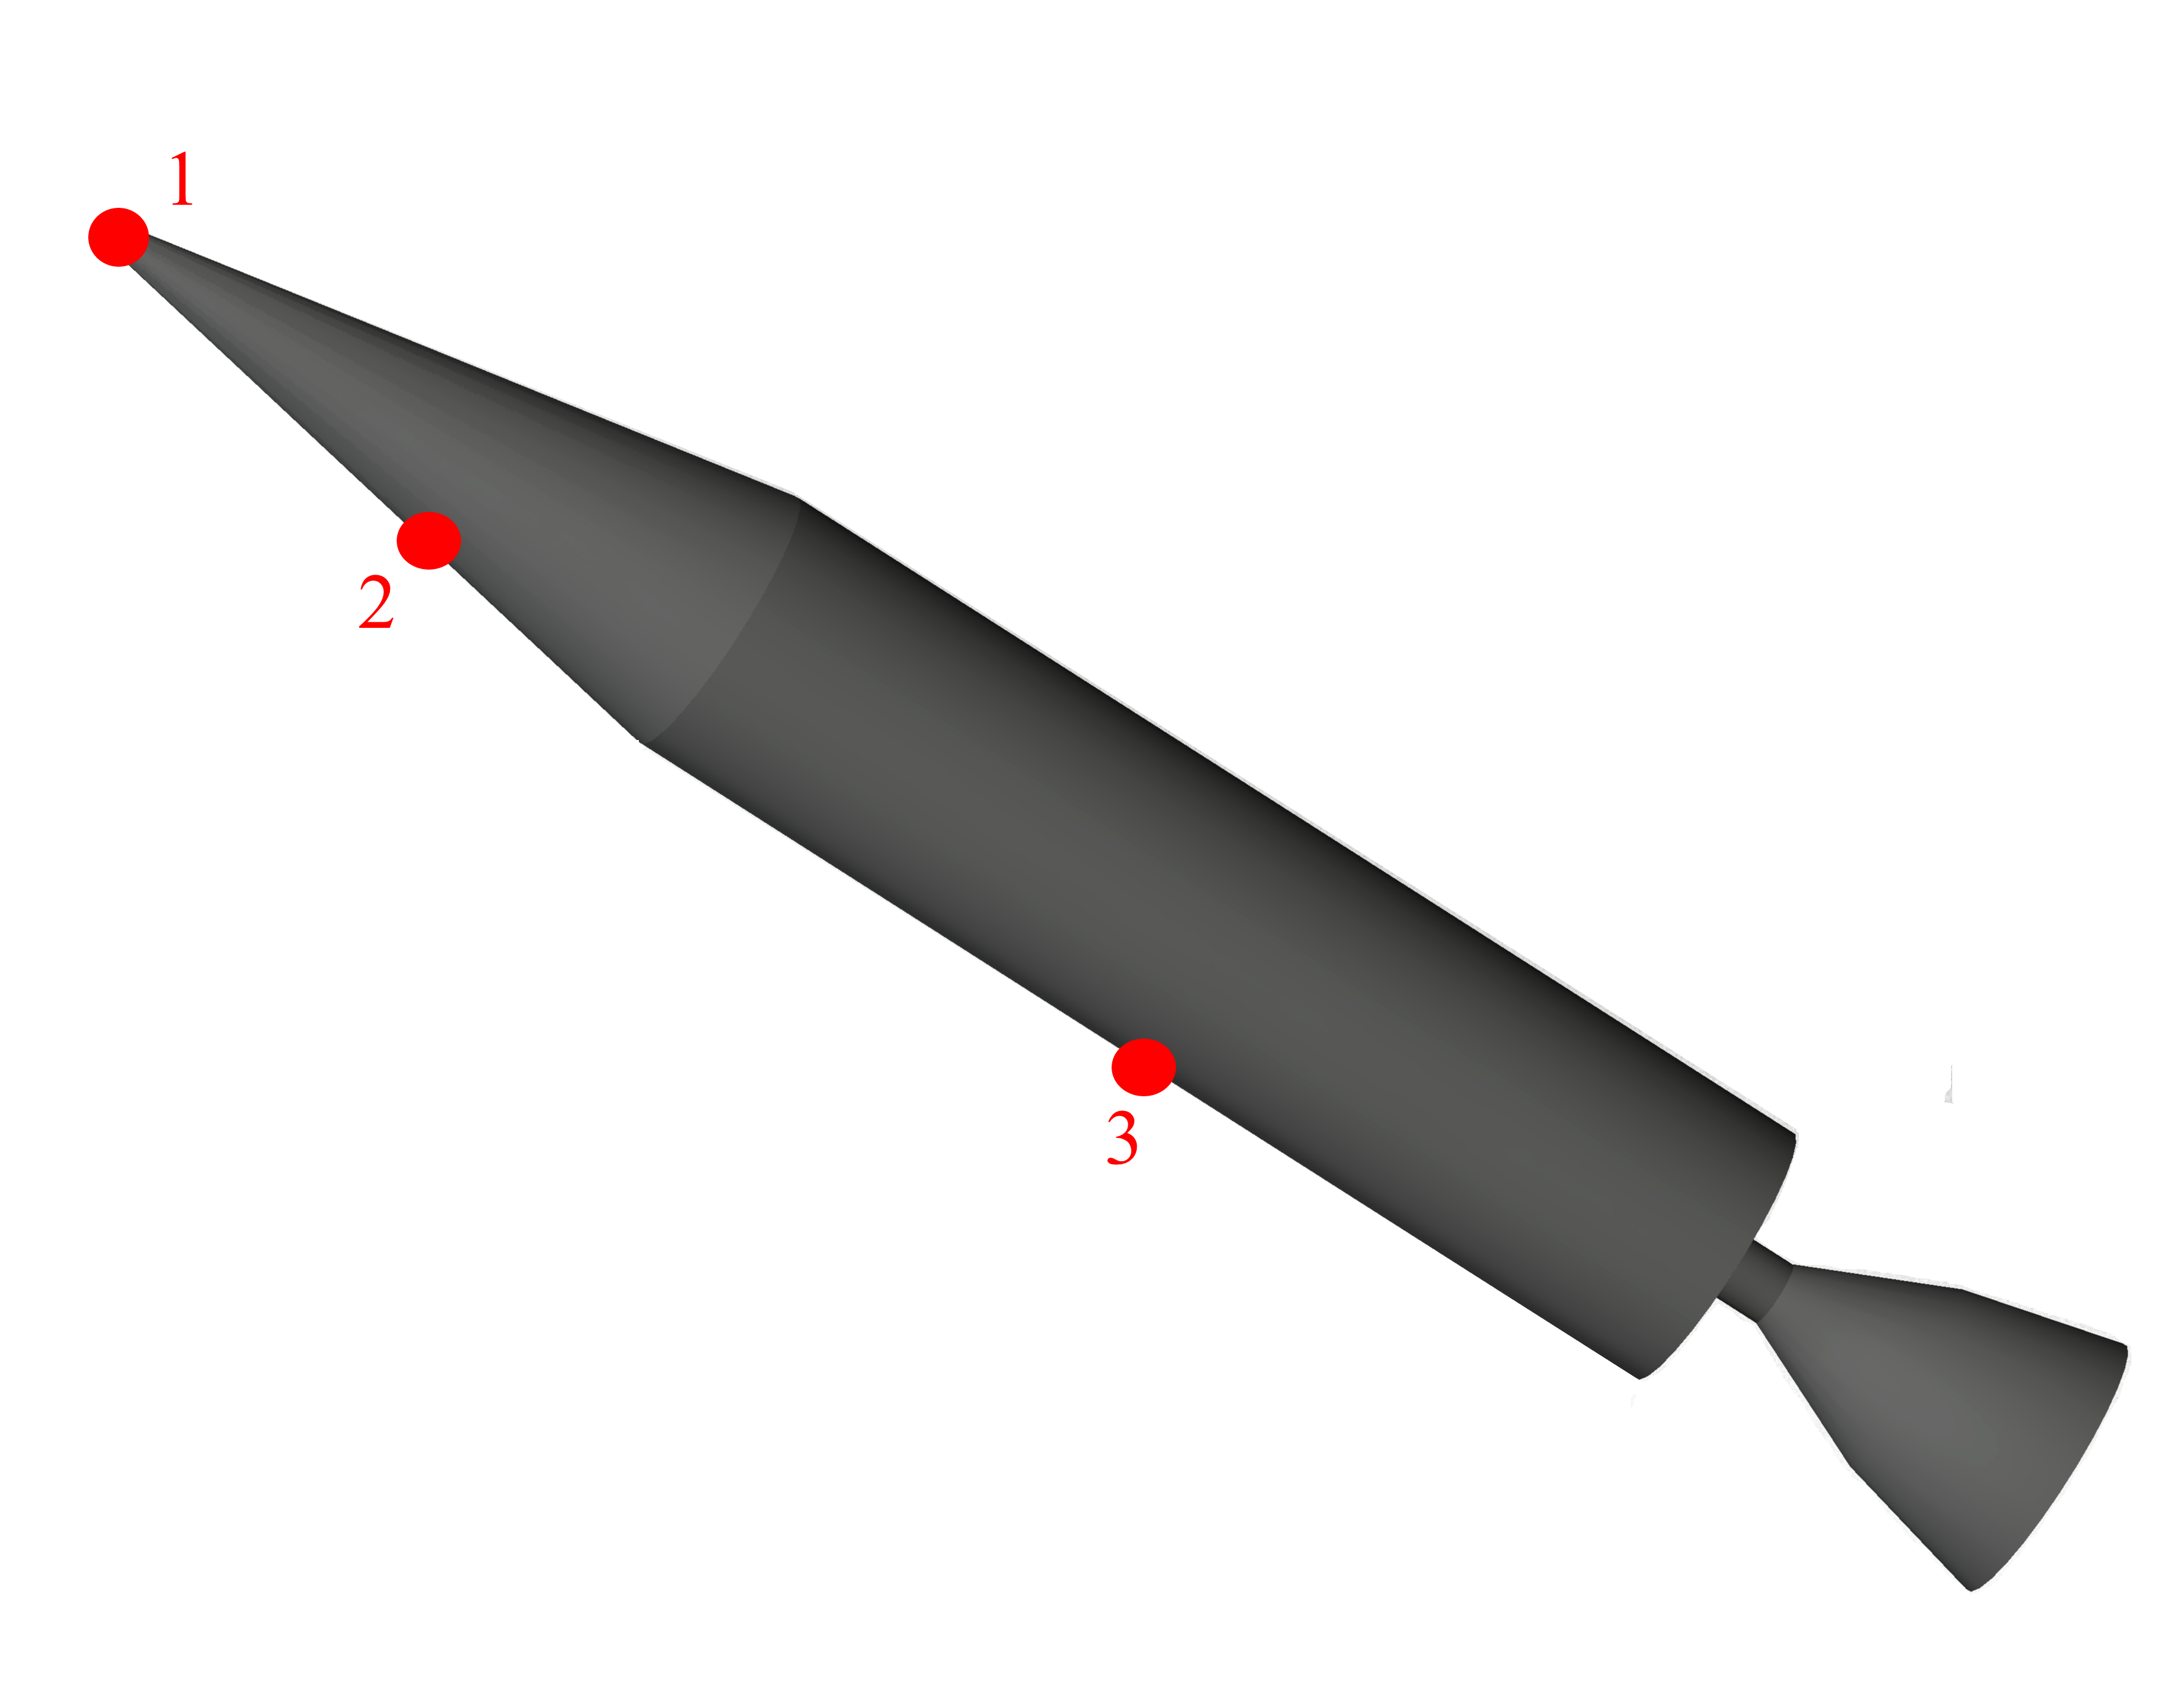
\includegraphics[width=0.9\linewidth]{figures/A1_uncertainty-analysis/Q_pos3}
\caption{The points examined on the third stage rocket.}
\end{subfigure}
\caption{The points chosen for thermal analysis, selected for the potential of high heat loading.}
\label{fig:Q_pos}
\end{figure}

The heat transfer at the stagnation point and leading edge of the wings, where the simple Reynold's analogy is not valid due to large pressure gradients in the flow\cite{HypersonicGas}, is estimated using semi-empirical correlations\cite{Dirkx}. At the stagnation point, the heat transfer is given by\cite{Dirkx}:
\begin{equation}
q_s = k_1\rho^{N_1}V^{N_2},
\end{equation}
where $N_1 = 0.5$ and $N_2 = 3$, and the constant $k$ is\cite{Dirkx}:
\begin{equation}
k_1 = \frac{1.83 \times 10^{-4}}{\sqrt{R_n}}(1-\frac{T_w}{T_{aw}}),
\end{equation}
where $R_n$ is the nose radius, $T_w$ is the wall temperature, and $T_{aw}$ is the adiabatic wall temperature.

The heating at the leading edge is given by a weighted average correlation between a stagnation point and a flat plate\cite{Dirkx,Tauber2008}:
\begin{equation}
q_{LE} = (\frac{1}{2}q_s^2 \cos^2(\Lambda) + q_{FP}^2 \sin^2(\Lambda))^{1/2},
\end{equation}
where $\Lambda$ is the wing sweep angle, and the equation for a flat plate is calculated assuming turbulent flow under 2962m/s as:
\begin{equation}
q_{FP} = k_2\rho^{N_3}V^{N_4},
\end{equation}
where $N_3 = 3.37$, $N_4 = 0.8$ and
\begin{equation}
k_2 = 3.35 \times 10^{-4} \cos^{1.78}(\theta) \sin^{1.6}(\theta) x_T^{-1/5} (\frac{T_w}{556})^{-1/4} (1 - 1.11\frac{T_w}{T_{aw}}),
\end{equation}
where $\theta$ is the flow incidence angle and $x_T$ is the distance along the body from the transition point\cite{Dirkx,Tauber2008}. For the purposes of the leading edge heating the transition point is assumed to be half the distance along the nose cone, and the transitional boundary layer length is assumed to be equal to the preceding laminar flow distance. Along with this assumption, the aeroheating is calculated at the start of the wing, providing an overall worst case scenario for the heating rate. Results for both best case and worst case transition points are provided in Appendix \textcolor{red}{XXX} and are shown to exhibit only \textcolor{red}{XXX}\% difference. As this is comparatively small and acknowledging the preliminary design nature (and associated design uncertainties) of the current project, we have opted to use the worst case assumption for estimating heat-transfer.



%\textcolor{red}{XXX Need to put in recognition for Alex \& Ingo for thermal stuff}


\section{Thermal Analysis of the Standard Trajectory}
 

\begin{figure}[ht]
	\begin{subfigure}{.5\textwidth}
		\centering
		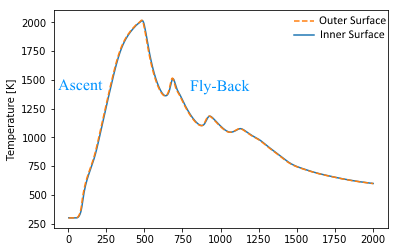
\includegraphics[width=0.99\linewidth]{figures/A1_uncertainty-analysis/TNoseReturn}
		\caption{The temperature time history at the nose (\textcolor{red}{1}.}
		
	\end{subfigure}
	\begin{subfigure}{.5\textwidth}
		\centering
		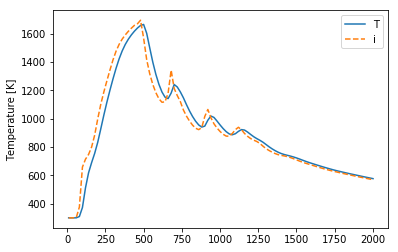
\includegraphics[width=0.99\linewidth]{figures/A1_uncertainty-analysis/TLEReturn}
		\caption{The temperature time history at the wing leading edge (\textcolor{red}{2}).}
		
	\end{subfigure}
	\begin{subfigure}{.5\textwidth}
		\centering
		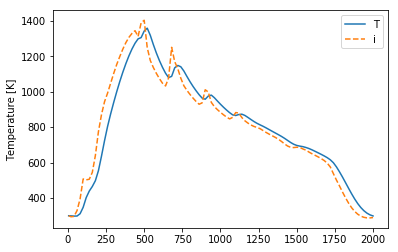
\includegraphics[width=0.99\linewidth]{figures/A1_uncertainty-analysis/TPos1Return}
		\caption{The temperature time history on the nose cone (\textcolor{red}{3}).}
		
	\end{subfigure}
	\begin{subfigure}{.5\textwidth}
		\centering
		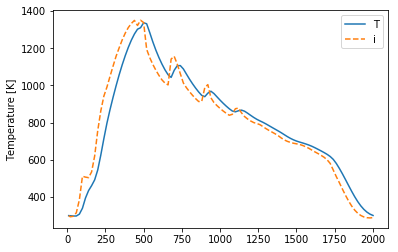
\includegraphics[width=0.99\linewidth]{figures/A1_uncertainty-analysis/TPos2Return}
		\caption{The temperature time history on the cowl (\textcolor{red}{4}).}
		
	\end{subfigure}
	\begin{subfigure}{.5\textwidth}
		\centering
		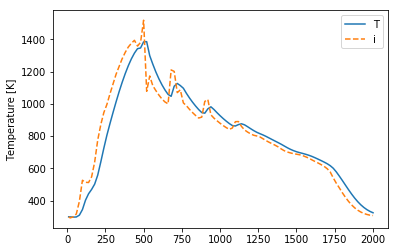
\includegraphics[width=0.99\linewidth]{figures/A1_uncertainty-analysis/TPos3Return}
		\caption{The temperature time history on the wing (\textcolor{red}{5}).}
		
	\end{subfigure}
	\begin{subfigure}{.5\textwidth}
		\centering
		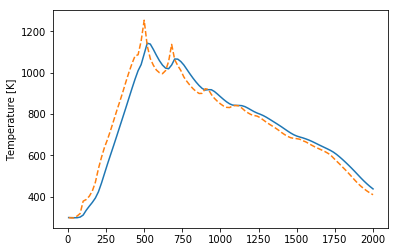
\includegraphics[width=0.99\linewidth]{figures/A1_uncertainty-analysis/TPos4Return}
		\caption{The temperature time history on the tail (\textcolor{red}{6}).}
		
	\end{subfigure}
	\caption{Temperature time histories on the scramjet accelerator.}
	\label{fig:TrajTemp}
\end{figure}


 
To determine the effectiveness of the SPARTAN's TPS system, a 1-D heat analysis is conducted.  
This heating calculation is implemented through the \textsf{uqTurbine} software package for 1-D heat transfer calculation, using the heat transfer calculated as defined in the previous section at each point along the trajectory. 
This gives an indication of the temperature at the specified points around the SPARTAN throughout its trajectory. 
Figures \ref{fig:TrajTemp} and \ref{fig:TrajTemp3} show the heat responses at the specified locations on the vehicles over the ascent trajectory of The SPARTAN. At the nose and leading edge it is assumed that there is no direct thermal connection to the internal insulation by the structure or TPS at the regions of maximum heat loads. The maximum heating in this area is therefore assumed to be limited by the properties of the TPS itself. The tungsten nose reaches 1947K, and the Carbon-Carbon wing leading edge reaches 1695K. These temperatures are well within the operational regimes of the materials, although they are outside the operational regime of the internal multilayer insulation. While it is outside the scope of this study to account for detailed internal design, the design of the stagnation region and leading edges along with appropriate structural support is likely to be a critical factor in the detailed design of The SPARTAN. These regions must be designed structurally so that the regions of high aerothermal and aerodynamic loads are able to be supported, while not exceeding the maximum operational temperature of the internal insulation close to the critical areas.  

\begin{figure}[ht]
	\begin{subfigure}{.495\textwidth}
		\centering
		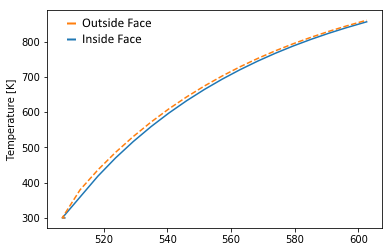
\includegraphics[width=0.99\linewidth]{figures/A1_uncertainty-analysis/TNose3}
		\caption{The temperature time history at the nose (\textcolor{red}{1}).}
		
	\end{subfigure}
	
	\begin{subfigure}{.495\textwidth}
		\centering
		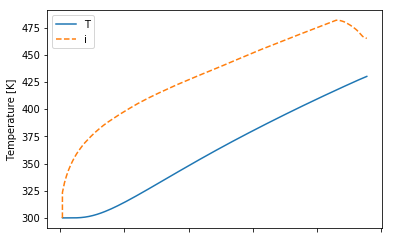
\includegraphics[width=0.99\linewidth]{figures/A1_uncertainty-analysis/T3onNose}
		\caption{The temperature time history on the nose cone (\textcolor{red}{2}).}
		
	\end{subfigure}
	
	\begin{subfigure}{.495\textwidth}
		\centering
		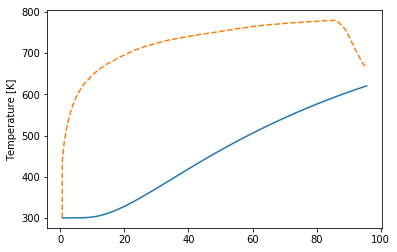
\includegraphics[width=0.99\linewidth]{figures/A1_uncertainty-analysis/T3Body}
		\caption{The temperature time history on the cylindrical body (\textcolor{red}{3}).}
		
	\end{subfigure}
	
	\caption{Temperature time histories on the third stage rocket with time.}
	\label{fig:TrajTemp3}
\end{figure}

On the body of the scramjet accelerator, the interior of the nose reaches a maximum of 1363K, the cowl 1361K, the wing 1337K, and the tail 1142K on the vehicle-facing edge. These temperatures are slightly greater than the 1000$^\circ$C external temperatures that the multilayer internal insulation has been tested for, where the back face of the insulation has been shown experimentally to keep temperatures to 300$^\circ$C\cite{Kourtides}. This indicates that the backface temperature of the insulation is likely to be slightly above 300$^\circ$C. This temperature is significantly less than the melting temperature of Aluminium, which is used for the internal structure, although it is within the range where conventional aluminium alloys begin to lose their mechanical strength. It is likely that a high temperature aluminium alloy would be required, at least in the regions of the internal structure that are close to the interface with the external insulation. In addition, these high temperatures will begin to reduce the mechanical strength of the internal insulation. This must be accounted for in the detailed internal design, so that the internal insulation does not fail when peak temperatures are reached. In this work it is assumed that the internal structure and insulation of the scramjet accelerator has been designed appropriately to account for regions of high heat load. 


%Max temps: T0 T1

%nose:
%1945.4358   1947.8085 

%LE
%1665.796    1695.4998 

%on body:
%Pos 1 - 1363.0571  1539.7696 
%Pos 2 - 1361.0127  1435.0191 
%pos 3 - 1337.0232  1350.7068 
%pos 4 - 1142.2337  1290.9281 


%third stage:
%nose tip: 874.80659 879.44989 

%Nose: 439.38044 472.50722 
%Body: 377.97737 397.55307 

% ingo thinks its probably best just to study the heating and not try to 'solve' it. eg how thick would the C-C shell need to be to resist heating? what might a heat limited trajectory look like? 

% Make argument that q limiting reduces the acceleration significantly - reducing pull up and payload - and that its probably more beneficial to find a better thermal protection system than q limiting

% need to really position this well, link to design, and to trajectories, explain how my trajectory results are still useful


% say something like 'the temperature is a bit over, but will need more detailed analysis to determine the best course of action, including possible the development of new internal insulation

% note that it is within the operational regime of the C-C




\section{Heating limited Trajectory}

To investigate the effects of limiting the maximum aerothermal heating on The SPARTAN's scramjet accelerator, the stagnation point heat flux is calculated in-loop using a cold wall approximation ($T_W = 0$).  


\textcolor{red}{XXX Not sure what I was doing here, might need to redo this to just a nominal heat flux limit? I think this limit was from when I was trying to bring the nose heating down a lot}

\begin{figure}[!ht]
\centering
\includegraphics[width=0.9\linewidth]{H:/github-home/LODESTAR-revisions/ArchivedResults/20190812T224102mode11qLim/FirstStageStandard}
\caption{}
\label{fig:FirstStageStandardqlim}
\end{figure}



\begin{figure}[!ht]
\centering
\includegraphics[width=0.9\linewidth]{H:/github-home/LODESTAR-revisions/ArchivedResults/20190812T224102mode11qLim/SecondStageStandard}
\caption{}
\label{fig:SecondStageStandardqlim}
\end{figure}

\begin{figure}[!ht]
\centering
\includegraphics[width=0.9\linewidth]{H:/github-home/LODESTAR-revisions/ArchivedResults/20190812T224102mode11qLim/ThirdStageStandard}
\caption{}
\label{fig:ThirdStageStandardqlim}
\end{figure}

\begin{figure}[!ht]
\centering
\includegraphics[width=0.9\linewidth]{H:/github-home/LODESTAR-revisions/ArchivedResults/20190812T224102mode11qLim/ReturnStandard}
\caption{}
\label{fig:ReturnStandardqlim}
\end{figure}

\begin{figure}[!ht]
\centering
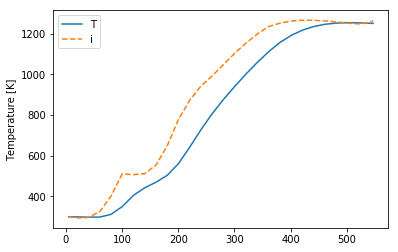
\includegraphics[width=0.7\linewidth]{figures/A1_uncertainty-analysis/TPos1-qlim}
\caption{}
\label{fig:TPos1-qlim}
\end{figure}

\begin{figure}[!ht]
\centering
\includegraphics[width=0.7\linewidth]{H:/github-home/LODESTAR-revisions/ArchivedResults/20190812T224102mode11qLim/HeatFluxStandard}
\caption{}
\label{fig:HeatFluxStandard}
\end{figure}


\section{TPS Design Exploration}

\section{Scramjet Accelerator}
-TPS thickness exploration

\textcolor{red}{XXX currently not converging}

--TPS thermal conductivity / density exploration

-possibly layers of different materials or new materials entirely


-active cooling exploration

17kW of cooling on the inner wall, activated during the scramjet accelerator stage, brings the internal nose temperature down to 1275.8K.
- redo this with multiple cooling rates - link to how internal structure might get too hot at critical areas

\begin{figure}[!ht]
\centering
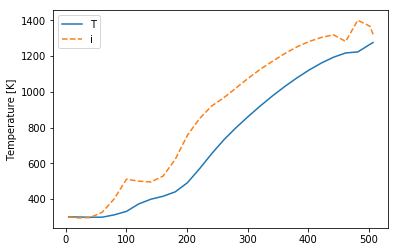
\includegraphics[width=0.7\linewidth]{figures/A1_uncertainty-analysis/TPos1-ActiveCooling}
\caption{}
\label{fig:TPos1-ActiveCooling}
\end{figure}







\section{Third Stage}

-- heat shield reduction due to pull-up?

-same sort of exploration as for scramjet stage?

\textcolor{red}{
\chapter{Modelling Uncertainties}
}

%-need to take into account that the error magnitudes estimated are only relative error (as above)

%-take into account that the values qoted for abeynayake paper are mean, and that the max errors are higher

This thesis aims to provide new insight into the operability and feasibility of multi-stage launch systems incorporating an air-breathing stage.
No such launch systems currently exist, and several of the technologies necessary for the successful operation of their systems and subsystems are in the research stage of development.
This means that that reliable performance data is not available, and while every effort has been made to apply accurate vehicle and subsystem models, it is acknowledged that several are not designed in detail or validated, and others had to be simplified during the modelling process. 
These simplifications and uncertainties are separated into two distinct parts; the simplifications that arise during vehicle design, and the uncertainties that arise from the modelling of the launch system performance. 

The design uncertainties that arise from simplifications during the design process affect the vehicle's geometry, structure and internal layout, and mass and mass-distribution. In this work the design process is necessarily simplified, and it is assumed that by making appropriate design choices the nominal vehicle can be constructed (i.e. it is assumed that the designer can achieve the representative design by selecting appropriate materials and layouts), and that the nominal vehicle is capable of flying an appropriate launch trajectory. In this stage it is important for the designer to be aware of the sensitivities and trade-offs between design input parameters and performance. These design simplifications are described in more detail in Section XXX, and their effects are expressed by the parameter-by-parameter sensitivity study conducted in Sections XXX and XXX. These sensitivity studies provide insights into how the design factors of the launch system impact on the performance of the launch system and the shape of the optimised trajectory.

The uncertainties that arise during the modelling of the performance of the launch system introduce differences between the actual launch system and the ``as-designed" nominal launch system. These uncertainties are inherent to the modelling assumptions in the aerodynamics and propulsion modelling of the launch system, in effect, even the most detailed designs will still suffer from many of the same modelling uncertainties as analysed (though with reduced margins). 
As the designer has no direct control over these variations between the ``as-designed" and actual vehicle, we need to rely on a-priori experience and a stochastic approach to quantify how the ultimate performance of the vehicle will be different to the ``as designed" simulations. The aim of this chapter is to apply a systematic approach to develop an understanding of how these uncertainties may affect the performance of the launch system. To consider this we first estimate the modelling uncertainties associated with the representative launch vehicle, and then conduct a reduced Monte-Carlo simulation (using Latin Hypercube sampling) to characterise how the modelling errors and simplifications affect the performance of an otherwise ``known" vehicle.




 







\section{Aerodynamic and Propulsion Simulation Uncertainties}


The purpose of this study is to determine the capabilities and performance of a multi-stage airbreathing launch system through the calculation and analysis of an optimal flight path. The calculation of an optimal flight path requires a large number of aerodynamic and propulsive simulations in order to cover the possible flight regimes of the launch system. In addition, the analysis of an optimal trajectory does not require high fidelity modelling techniques for useful information to be generated, because it is the general performance of the system that is of interest, rather than the specific performance of the design. Because of these factors, the launch system in this study is analysed using medium and low fidelity modelling techniques chosen for their fitness-for-purpose for optimal trajectory analysis, with an emphasis on computational efficiency as well as accuracy.
The uncertainties in the propulsive and aerodynamic properties of the launch system modelled in this work must be estimated, as there are no flight test or experimental results available for the representative launch system analysed in this study. In this section an estimate of the aerodynamic and propulsive uncertainties associated with the trajectory optimisations in this work is provided, and a Latin hypercube analysis is carried out to determine the variance in a sample trajectory optimisation and to assess the validity of the optimal trajectory results. 

\subsection{Aerodynamic Uncertainty}\label{sec:aerounc}




%\textcolor{red}{XXX I need to make sure this isnt contradicting my lit review at all, and should repeat some of this in my lit review.}

The aerodynamic coefficients of the SPARTAN in this work are calculated using an inviscid Euler solver, Cart3D, with a flat plate correction for the viscous forces. This is a medium fidelity method, which brings with it a significant associated uncertainty in the aerodynamics of the vehicle, particularly at subsonic and transonic conditions. Although the aerodynamics of the vehicle in this work are not experimentally validated, studies have previously compared Cart3D with experimental data for a number of geometries at various flight conditions. These experimental comparisons are utilised to estimate the uncertainty arising in the aerodynamic coefficients due to the use of Cart3D. These comparison studies do not usually correct for viscous forces, and so underpredict drag in almost all cases.



%- 'A Low Subsonic Study of the NASA N2A Hybrid Wing-Body Using an Inviscid Euler-Adjoint Solver' has error, but its too hard to estimate the values  from this.. . sagerman gives some specific pressure results, but only some. 

%\textcolor{red}{XXX be really careful here, the reviewer will know this paper inside out}
Abeynayake \& Agon assess two missile geometries; a conventional missile at transonic and supersonic speeds, and a non-conventional missile that has a cruise missile profile and includes small wings at subsonic speeds\cite{Abeynayake2013a}. The study by Abenayake and Agon estimates the magnitude of the uncertainty of Cart3D in a comparison to experimental results, although no viscous correction is included, and so the lack of a viscous component significantly affects the aerodynamic coefficients, particularly drag. The uncertainty magnitudes are estimated in relative error, normalised by the average value of data points between 0$^\circ$ and 10$^\circ$ angle of attack for drag, or the value at 10$^\circ$ angle of attack in the case of the lift and pitching moment coefficients\cite{Abeynayake2013a}. It is noted that these relative errors only give an indication of the accuracy of a specific tool\cite{Abeynayake2013a}. It is found that when compared to experimental results, Cart3D has a mean error in drag of 31.3\% for subsonic, 23.5\% for supersonic, and 18.0\% for transonic cases\cite{Abeynayake2013a} when compared to wind tunnel data for the non-conventional missile at angle of attack values between -10$^\circ$ and 10$^\circ$ in the subsonic regime, and the conventional missile at angles of attack of 0$^\circ$ to 10$^\circ$ in the transonic and supersonic regimes. The mean relative error in lift was found to be 16.5\% for subsonic, 1.3\% for supersonic, and 28.7\% for transonic cases\cite{Abeynayake2013a}, and the error in pitching moment 22.0\% for supersonic and 67.1\% for transonic cases, with no subsonic error given\cite{Abeynayake2013a}.
In this comparison study Cart3D was not able to match experimental trends closely in the subsonic and transonic regimes. Errors of up to 80.2\% in drag are observed in the subsonic regime for an unconventional missile geometry\cite{Abeynayake2013a}, although the drag error diminishes significantly at angle of attack values between -5$^\circ$ and 5$^\circ$. In the supersonic regime, Cart3D appears to closely match the experimental lift and drag trends, with an underprediction in the magnitude of the drag forces due to the absence of viscous forces. 
Cart3D had poor results when computing pitching moment, although it was occasionally able to match the magnitude of the pitching moment well Cart3D was not able to match the experimental pitching moment trends for either vehicle\cite{Abeynayake2013a}. The work by Abeynayake \& Agon indicates that the uncertainties associated with Cart3D are significant, particularly at angle of attack values greater than 5 in the subsonic and transonic regimes, and that it does not estimate pitching moment trends well. However, a portion of the uncertainty magnitudes are associated with the inviscid nature of Cart3D, particularly in the drag forces.


A study by Ward et al.\cite{Ward2018} compares Cart3D results to experimental results for a blunt body at hypersonic speeds, a lifting body vehicle at subsonic and supersonic speeds, and a hypersonic accelerator test geometry at hypersonic speeds. Ward et al. provide a method for viscous correction of the Cart3D results, and also compare this with experimental results, focusing on the amount that drag error is able to be corrected. In this study Cart3d was found to predict trends in drag coefficients well for all tested cases both subsonic and supersonic, although with a consistent underprediction of 15-25\% in drag coefficient due to a lack of viscous effects\cite{Ward2018}. When corrected for viscous effects, the drag coefficient was found to agree closely with the experimental results at supersonic and hypersonic speeds, with error reducing to less than 10\% for the hypersonic accelerator test vehicle, and less than 11\% for the lifting body at supersonic speed\cite{Ward2018}. Drag error at high angles of attack at subsonic speeds was still found to be large, at 38\%, however, at angles of attack under 5$^\circ$ the error reduced significantly, matching the experimental results to within 16\%. 

The Euclidean correction method outlined by A. Ward was utilised to correct the inviscid aerodynamic coefficients in this study, with viscous aerodynamics provided by A. Ward for this work. 
In addition, these two studies are used to inform the uncertainty margins in the aerodynamics of the representative launch system. Note that while the values reported by Abeynayake \& Agon\cite{Abeynayake2013a} are non-dimensionalised relative accuracies, it is assumed here that the values reported somewhat indicate the accuracy of Cart3D. 
For the lift uncertainties and the pitching moment at in the transonic and supersonic regimes, the uncertainty values are taken directly from the mean relative accuracies reported by Abeynayake \& Agon\cite{Abeynayake2013a}. The pitching moment error in the subsonic regime is not stated, so the average relative error for all Cart3D coefficients at subsonic speeds, 23\%, is used.
The subsonic uncertainty in the drag is estimated at a nominal value of 20\%, accounting for reduced uncertainty due to the low angle of attack of the launch system at subsonic speeds, which is shown to reduce error significantly.
This value is based primarily on the uncertainty determined by Ward et al.\cite{Ward2018} in the low subsonic regime at low angles of attack, with a slight increase due to the high uncertainties that are observed by Abeynayake \& Agon\cite{Abeynayake2013a}, which do not show evidence of a consistent trend due to a lack of viscous effects, though are again significantly reduced at low angles of attack. 
In the transonic case, Abenayake and Agon find that Cart3D is not capable of predicting the trends of the aerodynamic data well\cite{Abeynayake2013a}.
For this reason, the drag uncertainty in the transonic regime is set to 18\%, to match the mean value reported by Abenayake and Agon\cite{Abeynayake2013a}, as it is not evident that the lack of a viscous drag component produces a clear trend, and no corrected transonic cases are available. In the supersonic regime the ability of Cart3D to predict drag improves, and the lack of viscous effects causes an underprediction in drag while still matching experimental trends when uncorrected\cite{Abeynayake2013a,Ward2018}. The uncertainty in drag in the supersonic regime is set to 11\%, to match the maximum error observed after viscous correction by Ward et al.\cite{Ward2018}, assuming that the consistent underprediction observed by Abeynayake \& Agon\cite{Abeynayake2013a} is primarily due to a lack of viscous effects.
These uncertainty values are summarised in Table \ref{tab:AppendixUncertainty}, along with the uncertainties in the propulsion systems. 






%\subsubsection{Uncertainties Associated With Realistic Flight}

%The sources of variations between pre-flight predictions of hypersonic vehicles and actual flights are numerous, including modelling and experimental uncertainty, as well as on-the-day variations in the flight environment, vehicle and atmosphere. A study was carried out by Cobleigh\cite{X33} to develop an uncertainty model for the now discontinued X-33 SSTO demonstrator aircraft. The study by Cobleigh utilised comparisons of pre-flight aerodynamic estimates developed using either wind tunnel or computer modelling to flight test estimates for six lifting body aircraft, as well as the space shuttle, to estimate uncertainties in the aerodynamics of the X-33 from Mach 0.1 to 12. 
%-I have no way to convert the error from the coefficients to something useful. Also the lift coefficient errors that they have produced seem ridiculous compared to even their own aero coeffs in other papers? but they are saying its well predicted?




\subsection{Propulsion System Uncertainties}\label{sec:propunc}




\subsubsection{The Rocket Engines}
The propulsive properties of the rocket engines that power the first and third stages of the launch system are taken from the Falcon 1 Launch Vehicle Payload User's Guide\cite{Vehicle2008}, a document released by SpaceX that does not contain detailed information as to how the engine properties are calculated. It is assumed that the properties of the engines presented by SpaceX have been measured experimentally, and that the primary uncertainties associated with the rocket engine properties are experimental uncertainties. With no knowledge of the experimental facilities or processes used, it is necessary to estimate the experimental uncertainty through analysis of other experimental facilities, information that is generally sparse. Davidian, Diek and Chuang\cite{Davidian1987} assess the specific impulse uncertainty associated with high area ratio rocket tests at NASA Lewis Research centre, by propagating an "exhaustive" list of possible error sources. The test facility was found to be capable of measuring specific impulse to within 1.30\%, thrust to within 1.12\%, and mass flow rate to within 0.72\%. These propagated uncertainty values assumed that there was no bias errors, and that calibration had no error prior to testing. 
The uncertainty in the specific impulse of 1.30\% is used as the rocket engine performance uncertainty for the purposes of this study, assuming that the testing that has been carried out on the Merlin 1-C and Kestrel engines has the same error margins as the NASA Lewis Research Centre facilities. 

\subsubsection{The Scramjet Engine}
%Quasi-One-Dimensional Model of Hydrogen-Fueled Scramjet Combustors". These are the studies that the engine models were likely tuned off 

%Ingo says that I might need to ballpark a number, say 25\%, but that it could be much higher, even 50\% in his optinion. I will need to be very clear here. 

%\textcolor{red}{XXX check with michael about the experimental corrections, is there a reference for it?}
%-ask michaael if crest database has experiomental results- ingo thinks that 1D ANalysis is tuned using ground test data. In this case it doesnt make much sense to work out uncertainty from ground test data.
The C-REST engines are modelled in this work using a dataset developed using a combination of high-fidelity CFD, and quasi 1-D analysis, tuned using experimental results\cite{Jazra2010}. Estimating the error in this model in comparison to a realistic, flight capable scramjet is not feasible, due to the lack of flight test data or full-scale engine ground testing for scramjet engines in the public domain. For the purposes of this study a nominal uncertainty of 25\% is associated with the specific impulse of the scramjet engines based on the experience of the Author's colleagues and supervisors at The University of Queensland's Centre for Hypersonics. This is an estimated uncertainty margin, and it is possible that the uncertainty margin may be higher than this estimated value. However it is probable that if there is errors larger than 25\% in the performance modelling of the scramjet engines, then the design of the system may have to change considerably to be feasible. For this reason, the uncertainty margin of the scramjet specific impulse is kept at 25\% for payload-to-orbit uncertainty margin calculations, although it is acknowledged that major unforseen modelling or experimental errors may cause design changes to be necessary or lead to the infeasibility of the system as a whole. 


\subsection{Quantification of Aerodynamic and Propulsion Uncertainty Effects}


\subsubsection{Quantification of Uncertainty Magnitudes}

The uncertainty margins of the aerodynamic and propulsive data for the representative launch system analysed in this study are shown in Table \ref{tab:AppendixUncertainty}. These uncertainty margins have been developed based on the errors described in the studies analysed Sections \ref{sec:aerounc} \& \ref{sec:propunc}. 

%-note that it is assumed that only the moments on the spartan are affected, and not the flaps

\begin{table}
	\centering
	\begin{tabular}{|c|c|c|c|}
		\hline  Uncertainty & Subsonic & Transonic  & Supersonic/Hypersonic \\ 
		\hline  1$^{st}$ \& 3$^{rd}$ Stage $I_{SP}$ & 1.3\% & 1.3\% &  1.3\% \\ 
		\hline  Scramjet $I_{SP}$ & - & - &  25\% \\ 
		\hline   $C_L$ & 16.5\% & 28.7\% & 1.3\% \\  
		\hline   $C_D$ & 20\% & 18\% & 11\% \\  
		\hline   $C_M$  & 23\% & 67.1\% &  22.0\% \\ 
		\hline 
	\end{tabular}
	\caption{The uncertainty margins associated with the aerodynamic and propulsive modelling of The SPARTAN.}
	\label{tab:AppendixUncertainty}
\end{table}


	%\hline  Third Stage $C_a$ & - & - &  34.5\% \\ 
	%\hline  Third Stage $C_n$ &  -& - & 8.9\% \\ 
	%\hline  Third Stage $C_M$ & - & - & 17.4\%  \\ 
	%\hline  Third Stage $I_{SP}$ & - & - & 1.3\%  \\ 

\subsubsection{Variation Study}
In order to quantify the effects of the uncertainty in the aerodynamic and propulsion models, a Monte Carlo variation study is carried out using a Latin Hypercube Sampling technique. A sample size of 85 runs was used, distributed using Matlab's \textsf{lhsdesign} function. 
%-2 sigma variation? normalised spread?

-running more LHC tests to add to this to see if it is a normal dist
\begin{figure}[ht]
\centering
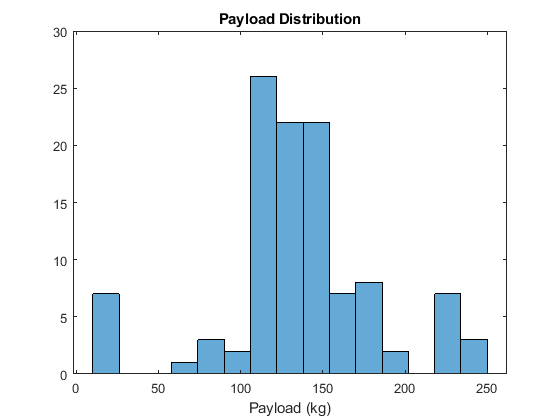
\includegraphics[width=0.7\linewidth]{figures/A1_uncertainty-analysis/LHC}
\caption{The distribution of optimised payload-to-orbit values over the range of LHC determined samples.}
\label{fig:LHC}
\end{figure}



\subsection{Atmospheric Variations}

The Earth's atmosphere varies significantly depending on location, and over time. As such, the atmosphere into which The SPARTAN is launched may be considerably different to the atmosphere that is being modelled in this work. 
The variations in the properties of the atmosphere with geography or time may affect the aerodynamic and engine performance of the launch system significantly, and change the altitude at which maximum dynamic pressure is reached. These variations may have significant impact on the aerodynamic and aerothermal performance of the launch system at a particular altitude, as well as the performance of the propulsion systems of the launch system, particularly the scramjet engines. 
This study uses the U.S Standard Atmosphere 1976 model\cite{Administration1976} to calculate the properties of the atmosphere during simulations. The U.S Standard Atmosphere 1976 is based on a collection of data from sites across America, Brazil, Australia, and Russia, with values calculated for annual mean properties at an interpolated latitude of 45$^\circ$\cite{Administration1976}. The properties that are calculated using this atmosphere are subject to seasonal variability, as well as variability due to geographic position. Figure \ref{fig:AtmosphericVariation} shows the variation in temperature and pressure in the 1976 U.S Standard Atmosphere model with altitude. In the higher latitudes maximum and minimum temperatures at altitudes below 25km are seasonal, however at higher altitudes semi-annual and biennial oscillations have a large influence\cite{Administration1976}. The variations shown do not occur at the same time in the same envelopes of the atmosphere; warm temeratures at the surface are associated with cold temperatures near the tropopause, and temperatures near the stratopause are negatively correlated with temperatures near the mesopause\cite{Administration1976}. These oscillations are particularly important in the equatorial regions, where the seasonal variation in temperature is smallest. 

\begin{figure}[ht]
	\centering
	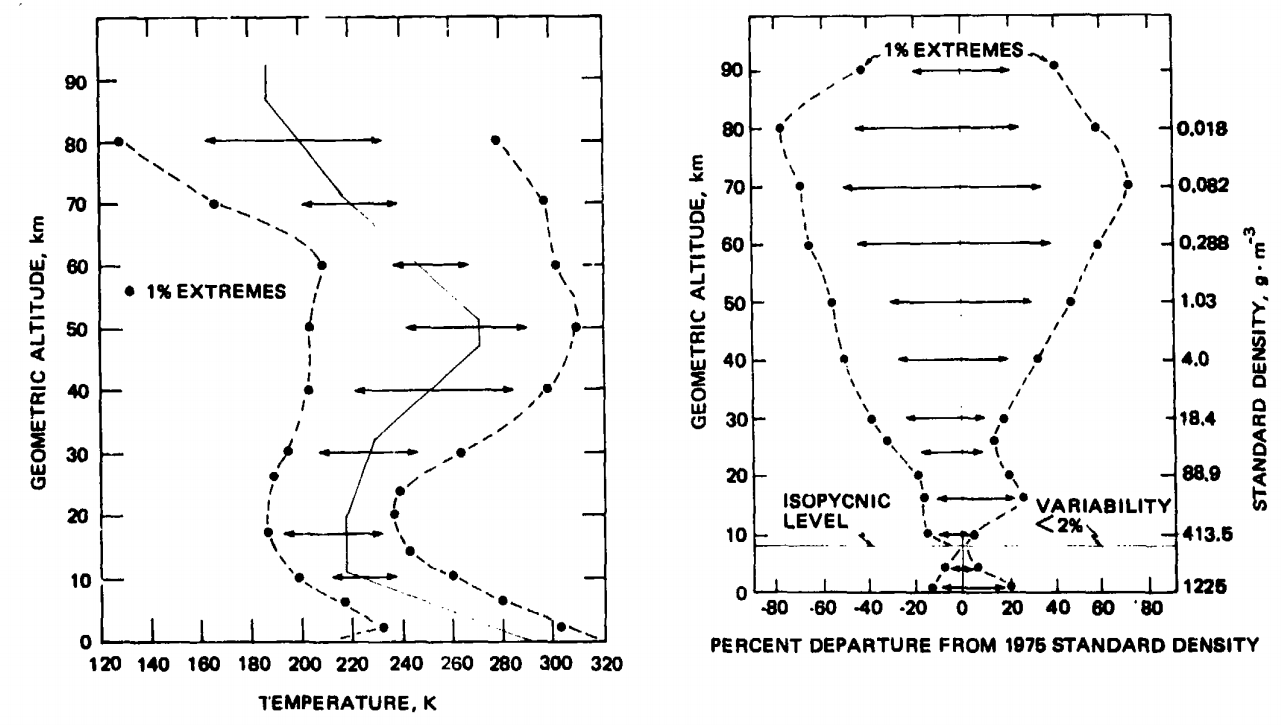
\includegraphics[width=0.8\linewidth]{figures/A1_uncertainty-analysis/AtmosphericVariation}
	\caption{Variation in temperature and density in the 1976 U.S Standard Atmosphere Model\cite{Administration1976}. Arrows indicate lowest and highest mean monthly values obtained at any location, and dashed lines indicate one-percent extremes.}
	\label{fig:AtmosphericVariation}
\end{figure}

The effects of atmospheric variation are quantified by modelling the 1976 U.S Standard Atmosphere model to take into account the maximum and minimum variations shown in Figure \ref{fig:AtmosphericVariation}. It is assumed that the conditions at the surface compared to the tropopause vary inversely, as well as the conditions of the stratopause compared to the mesopause, as indicated in Figure \ref{fig:AtmosphericVariation}. The conditions in the stratosphere are assumed to vary linearly between the conditions at the tropopause and stratopause. It is also assumed that density varies inversely to temperature, so that maximum temperature conditions correspond to minimum density. As such, there are two conditions at ground level, and two conditions at stratopause to be investigated. 

\textcolor{red}{XXX need to add standard traj to this}

\begin{tabular}{l c c c c} 
	\hline \textbf{Trajectory Condition}
	& MinTGroundMinTStrat
	& MaxTGroundMinTStrat
	& MinTGroundMaxTStrat
	& MaxTGroundMaxTStrat
	\\
	\hline \textbf{Payload to Orbit (kg)}
	& \textbf{\PayloadToOrbitMinTGroundMinTStrat}
	& \textbf{\PayloadToOrbitMaxTGroundMinTStrat}
	& \textbf{\PayloadToOrbitMinTGroundMaxTStrat}
	& \textbf{\PayloadToOrbitMaxTGroundMaxTStrat}
	\\
	\textbf{Payload Variation (\%)}
	& \PayloadVarMinTGroundMinTStrat
	& \PayloadVarMaxTGroundMinTStrat
	& \PayloadVarMinTGroundMaxTStrat
	& \PayloadVarMaxTGroundMaxTStrat
	\\
	\textbf{Total $\eta_{exergy}$ (\%)}
	& \textbf{\totalExergyEffMinTGroundMinTStrat}
	& \textbf{\totalExergyEffMaxTGroundMinTStrat}
	& \textbf{\totalExergyEffMinTGroundMaxTStrat}
	& \textbf{\totalExergyEffMaxTGroundMaxTStrat}
	\\
	\hline 
	\textbf{1$^{st}$ Stage $\eta_{exergy}$ (\%)}
	& \textbf{\firstExergyEffMinTGroundMinTStrat}
	& \textbf{\firstExergyEffMaxTGroundMinTStrat}
	& \textbf{\firstExergyEffMinTGroundMaxTStrat}
	& \textbf{\firstExergyEffMaxTGroundMaxTStrat}
	\\
	\textbf{Separation Alt, 1$\rightarrow$2 (km)}
	& \firstsecondSeparationAltMinTGroundMinTStrat
	& \firstsecondSeparationAltMaxTGroundMinTStrat
	& \firstsecondSeparationAltMinTGroundMaxTStrat
	& \firstsecondSeparationAltMaxTGroundMaxTStrat
	\\
	\textbf{Separation v, 1$\rightarrow$2 (m/s)}
	& \firstsecondSeparationvMinTGroundMinTStrat
	& \firstsecondSeparationvMaxTGroundMinTStrat
	& \firstsecondSeparationvMinTGroundMaxTStrat
	& \firstsecondSeparationvMaxTGroundMaxTStrat
	\\
	\textbf{Separation $\gamma$, 1$\rightarrow$2 (deg)}
	& \firstsecondSeparationgammaMinTGroundMinTStrat
	& \firstsecondSeparationgammaMaxTGroundMinTStrat
	& \firstsecondSeparationgammaMinTGroundMaxTStrat
	& \firstsecondSeparationgammaMaxTGroundMaxTStrat
	\\
	\hline 
	\textbf{2$^{nd}$ Stage $\eta_{exergy}$ (\%)}
	& \textbf{\secondExergyEffMinTGroundMinTStrat}
	& \textbf{\secondExergyEffMaxTGroundMinTStrat}
	& \textbf{\secondExergyEffMinTGroundMaxTStrat}
	& \textbf{\secondExergyEffMaxTGroundMaxTStrat}
	\\
	\textbf{Separation Alt, 2$\rightarrow$3 (km)}
	& \secondthirdSeparationAltMinTGroundMinTStrat
	& \secondthirdSeparationAltMaxTGroundMinTStrat
	& \secondthirdSeparationAltMinTGroundMaxTStrat
	& \secondthirdSeparationAltMaxTGroundMaxTStrat
	\\
	\textbf{Separation $v$, 2$\rightarrow$3 (m/s)}
	& \secondthirdSeparationvMinTGroundMinTStrat
	& \secondthirdSeparationvMaxTGroundMinTStrat
	& \secondthirdSeparationvMinTGroundMaxTStrat
	& \secondthirdSeparationvMaxTGroundMaxTStrat
	\\
	\textbf{Separation $\gamma$, 2$\rightarrow$3 (deg)}
	& \secondthirdSeparationgammaMinTGroundMinTStrat
	& \secondthirdSeparationgammaMaxTGroundMinTStrat
	& \secondthirdSeparationgammaMinTGroundMaxTStrat
	& \secondthirdSeparationgammaMaxTGroundMaxTStrat
	\\
	\textbf{2$^{nd}$ Stage Flight Time (s)}
	& \secondFlightTimeMinTGroundMinTStrat
	& \secondFlightTimeMaxTGroundMinTStrat
	& \secondFlightTimeMinTGroundMaxTStrat
	& \secondFlightTimeMaxTGroundMaxTStrat
	\\
	\textbf{2$^{nd}$ Stage Distance Flown (km)}
	& \SecondDistMinTGroundMinTStrat
	& \SecondDistMaxTGroundMinTStrat
	& \SecondDistMinTGroundMaxTStrat
	& \SecondDistMaxTGroundMaxTStrat
	\\
	\textbf{2$^{nd}$ Stage Return Fuel (kg)}
	& \returnFuelMinTGroundMinTStrat
	& \returnFuelMaxTGroundMinTStrat
	& \returnFuelMinTGroundMaxTStrat
	& \returnFuelMaxTGroundMaxTStrat
	\\
	\textbf{2$^{nd}$ Stage Return Distance (km)}
	& \returnDistMinTGroundMinTStrat
	& \returnDistMaxTGroundMinTStrat
	& \returnDistMinTGroundMaxTStrat
	& \returnDistMaxTGroundMaxTStrat
	\\
	\hline 
	\textbf{3$^{rd}$ Stage $\eta_{exergy}$ (\%)}
	& \textbf{\thirddExergyEffMinTGroundMinTStrat}
	& \textbf{\thirddExergyEffMaxTGroundMinTStrat}
	& \textbf{\thirddExergyEffMinTGroundMaxTStrat}
	& \textbf{\thirddExergyEffMaxTGroundMaxTStrat}
	\\
	\textbf{3$^{rd}$ Stage $t$, $q >$ 5kpa (s)}
	& \thirdqOverFiveMinTGroundMinTStrat
	& \thirdqOverFiveMaxTGroundMinTStrat
	& \thirdqOverFiveMinTGroundMaxTStrat
	& \thirdqOverFiveMaxTGroundMaxTStrat
	\\
	\textbf{3$^{rd}$ Stage max $\alpha$ (deg)}
	& \thirdmaxAoAMinTGroundMinTStrat
	& \thirdmaxAoAMaxTGroundMinTStrat
	& \thirdmaxAoAMinTGroundMaxTStrat
	& \thirdmaxAoAMaxTGroundMaxTStrat
	\\
	\textbf{3$^{rd}$ Stage Fuel Mass (kg)}
	& \thirdmFuelMinTGroundMinTStrat
	& \thirdmFuelMaxTGroundMinTStrat
	& \thirdmFuelMinTGroundMaxTStrat
	& \thirdmFuelMaxTGroundMaxTStrat
	\\
	\hline 
\end{tabular} 



\chapter{Examples and Verification}

\section{Example - Brachistochrone Problem}

This section describes a short example of an optimal control problem solved in GPOPS-II. The purpose of this example is to demonstrate the effectiveness of the pseudospectral method and GPOPS-II, and to provide a simple example case to establish the terminology of an optimal control problem.  


The brachistochrone (from the Greek for 'shortest time') problem is a simple optimal control problem, which describes a ball rolling in two dimensions under gravity. The objective is to find the curve of descent which will minimise the time from point \textit{a}, where the ball is at rest, to point \textit{b}. It is assumed that gravity is constant and that there is no forces other than gravity acting on the ball. 
The analytical solution of this problem can be computed using the Euler-Lagrange equation as the equations describing a cycloid:

$x = A(\theta + \sin\theta) $,

$y=A(1 - \cos\theta)$

This problem is included within GPOPS-2 as an example problem, and has been solved to illustrate the GPOPS-2 solution set-up\cite{Rao2010}. Table \ref{tab:brachistochrone} describes the set-up of the optimal control problem in GPOPS-2. The dynamic equations for the Brachistochrone problem are:

$\dot{x} = v*cos(u)$,

$\dot{y} = v*sin(u)$,

$\dot{v} = g*sin(u)$.

\noindent These equations are provided to GPOPS-2 as the time-variant system model in this form. The control variable is set to be the descent angle. The initial constraints are defined to initiate the ball at rest at the origin, and the terminal constraints are defined to terminate the problem at coordinates of [2,2]. The cost is set to minimum time, so that the solution will be the descent angle which minimises the time to get from the initial position, to the end position. 

\begin{table}
	\centering
	\begin{tabular}{|c|c|}
		\hline Primal Variables  & x Position\\& y Position\\& Velocity\\ 
		\hline Control Variables  & Angle of Descent\\ 
		\hline Initial Constraints  & Velocity\\ & x Position\\ & y Position\\
		\hline Terminal Constraints &  x Position\\ & y Position\\
		\hline Path Constraints & None \\ 
		\hline Target Cost & Minimum Time \\ 
		\hline 
	\end{tabular} 
	\caption{Optimisation setup of the Brachistochrone problem. }
	\label{tab:brachistochrone}
\end{table}


The GPOPS-2 solution to the Brachistochrone problem is shown in Figure \ref{fig:Brachistochrone}, matching the analytical solution almost exactly. This is expected in this case, as the dynamics of the basic Brachistochrone problem are very simple. As the dynamics become more complex, it is no longer possible to obtain an analytical solution.  

\begin{figure}[ht]
	\centering
	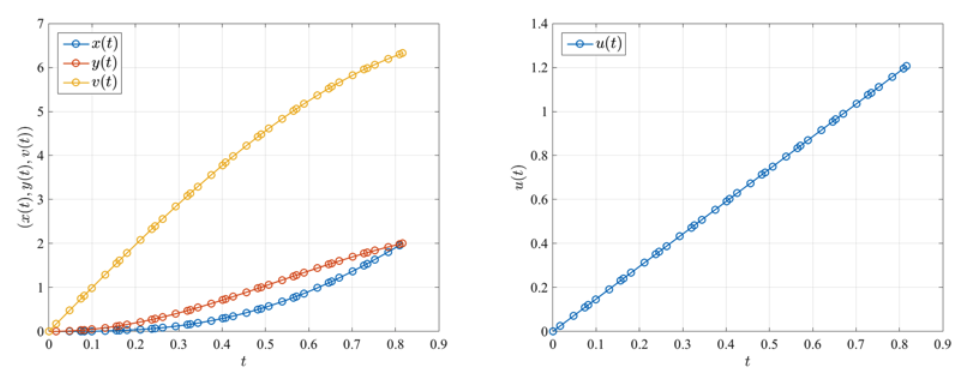
\includegraphics[width=0.9\linewidth]{figures/4_LODESTAR/Brachistochrone}
	\caption{The solution to the Brachistochrone problem, solved in GPOPS-2\cite{Rao2010}.}
	\label{fig:Brachistochrone}
\end{figure}




\textcolor{red}{\section{Example - Space Shuttle Reentry}}
\textcolor{red}{XXX I havent been able to find any good trajectories for comparison, that offer me the ability to recreate them..}
\textcolor{red}{XXX this is not quite the same as the GPOPS example, more similar to my dynamics}

This section describes an optimised shuttle reentry trajectory problem, taken from the textbook 'Practical Methods for Optimal Control and Estimation Using Nonlinear Programming' by Betts\cite{Betts2009}, which has been simulated in GPOPS-2 to illustrate the capabilities of GPOPS-2 when applied to a complex aerodynamic problem of an existing vehicle. The optimisation of the space shuttle reentry is relevant due to the large flight regime and long time period being simulated, which leads to a complex, extremely sensitive optimal control problem\cite{Betts2009}, similar in a simplified manner to the problem being solved in this work. The shuttle reentry problem is highly nonlinear and intractable to simple optimisation methods\cite{Betts2009}, making it suitable for illustrating the robustness of GPOPS-2 for aerospace problems of this type. 
The space shuttle reentry problem aims to maximise crossrange during reentry, with two cases; unconstrained, and limited by a simple heating rate constraint. The example in this section uses the vehicle model exactly as defined by Betts\cite{Betts2009} for comparison purposes, however the problem is formulated in a simplified version of the coordinate system that is used in the rest of this work. 


\subsection{Problem Formulation}

The dynamics of the space shuttle are defined exactly similarly to those in the problem designed by Betts\cite{Betts2009}, using a simplified model that neglects the rotation of the Earth and the tangential component of gravity:

\begin{equation}
\dot{r} = v \sin \gamma,
\end{equation}

\begin{equation}
\dot{\xi} = \frac{v\cos \gamma \cos \zeta}{r \cos \phi},
\end{equation}

\begin{equation}
\dot{\phi} = \frac{v\cos\gamma\sin\zeta}{r},
\end{equation}
\begin{equation}
\dot{\gamma} = \frac{L \cos\eta}{mv} + (\frac{v}{r}-\frac{g}{v})\cos\gamma,
\end{equation}
\begin{equation}
\dot{v} = \frac{D}{m}-g\sin\gamma,
\end{equation}
\begin{equation}
\dot{\zeta} = \frac{L  \sin\eta}{mv \cos \gamma}-\frac{v}{r}\tan\phi\cos\gamma\cos\zeta.
\end{equation}

The aerodynamics of the vehicle are modelled using simple correlations, where $C_L = −0.20704 + 0.029244\alpha$, and $C_D = 0.07854 -0.61592\times10^{-2}\alpha^2 + 0.621408\times10^{-3}\alpha^3$. The density is modelled as exponentially decaying, $\rho = 1.2255708354e^{-h/7254}$, and the gravity is modelled by an inverse square law, $g = \frac{\mu}{r^2}$.
The space shuttle initial conditions are set as follows\cite{Betts2009}, to simulate the entry of the shuttle into the upper atmosphere:
\begin{table}[H]
	\centering
\begin{tabular}{c c}
  $h_0$ =  79248m, & $v_0$ = 7803m/s, \\ 
  $\gamma_0$ =  -1$^\circ$, & $\phi_0$ =  0$^\circ$,\\ 
 $\xi_0$ =  0$^\circ$, & $\zeta_0$ =  0$^\circ$,\\ 
\end{tabular} 
\end{table}
and the end conditions are set as follows\cite{Betts2009}, to match the terminal area energy management interface:
\begin{table}[H]
	\centering
	\begin{tabular}{ c c c}
		   $h_f$ =  24384m, &  $v_f$ =762m/s, & $\gamma_f$ =  -5$^\circ$.\\ 
		
		
	\end{tabular} 
\end{table}

The problem is set to maximise crossrange from the initial point, which in this case is equivalent to maximising latitude:

\begin{equation}
J = -\phi_f.
\end{equation}

\subsection{Unconstrained Result}
The shuttle rentry crossrange maximisation problem is optimised in GPOPS-2, with result time histories shown in Figures \ref{fig:SpaceShuttleNoq1} and \ref{fig:SpaceShuttleNoq2}. The shuttle follows a 'skipping' trajectory, with an initially large bank angle that changes the heading of the vehicle rapidly in the early stages of reentry. The skips serve to maximise the range of the space shuttle's flight, and they are controlled by the angle of attack of the vehicle. The solution computed in GPOPS-2 matches the result computed by Betts\cite{Betts2009}, with the shape of the trajectories being close to identical. A maximum crossrange of 34.18$^\circ$ is achieved, a difference of 0.11\% when compared to the solution computed by Betts\cite{Betts2009}. This result is indicative of the ability of GPOPS-2 to compute highly sensitive optimal control problems for aerospace vehicles. 


\begin{figure}[H]
\centering
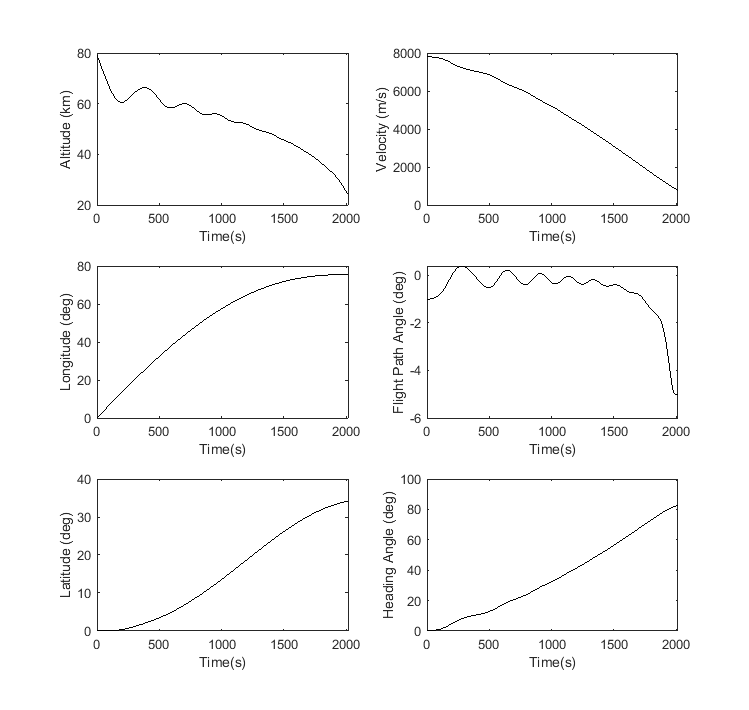
\includegraphics[width=0.7\linewidth]{figures/A1_uncertainty-analysis/SpaceShuttleNoq1}
\caption{}
\label{fig:SpaceShuttleNoq1}
\end{figure}
\begin{figure}[H]
\centering
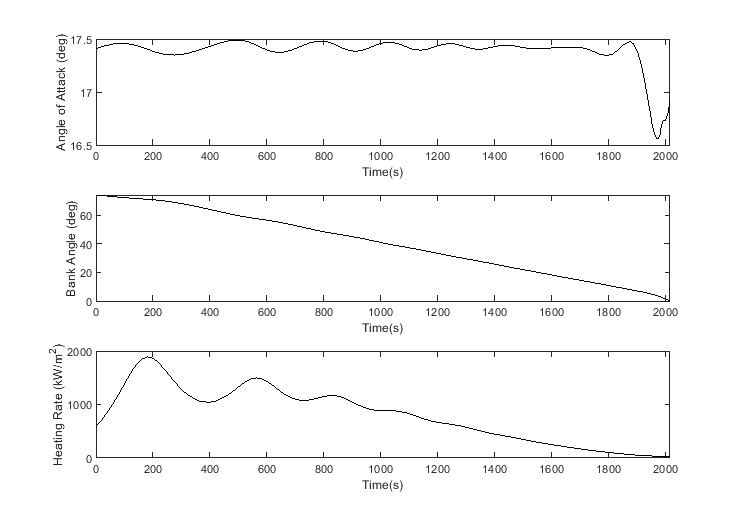
\includegraphics[width=0.7\linewidth]{figures/A1_uncertainty-analysis/SpaceShuttleNoq2}
\caption{}
\label{fig:SpaceShuttleNoq2}
\end{figure}


\subsection{Heating Rate Limited Result}
%\textcolor{red}{XXX Need to find a way to denote heating rate thats not q}
The heating rate of the space shuttle is limited during descent, to illustrate the ability of GPOPS-2 to deal with complex inequality constraints. The leading edge heating is approximated using a simplified empirical model, so that $q = q_aq_r$, where $q_r = 17700\sqrt{\rho}(0.0001v)^{3.07}$ and $q_a = 1.0672181 -0.19213774\times10^{-1}
\alpha + 0.21286289\times10^{-3}\alpha^2 -0.10117249\times10^{-5}\alpha^3$. The trajectory is successfully optimised in the presence of this complex inequality, once again showing a near identical trajectory to the optimised solution calculated by Betts\cite{Betts2009}. The maximum crossrange is reduced to 30.70$^\circ$, a difference of 0.25\% to the solution calculated by Betts\cite{Betts2009}.

\begin{figure}[H]
\centering
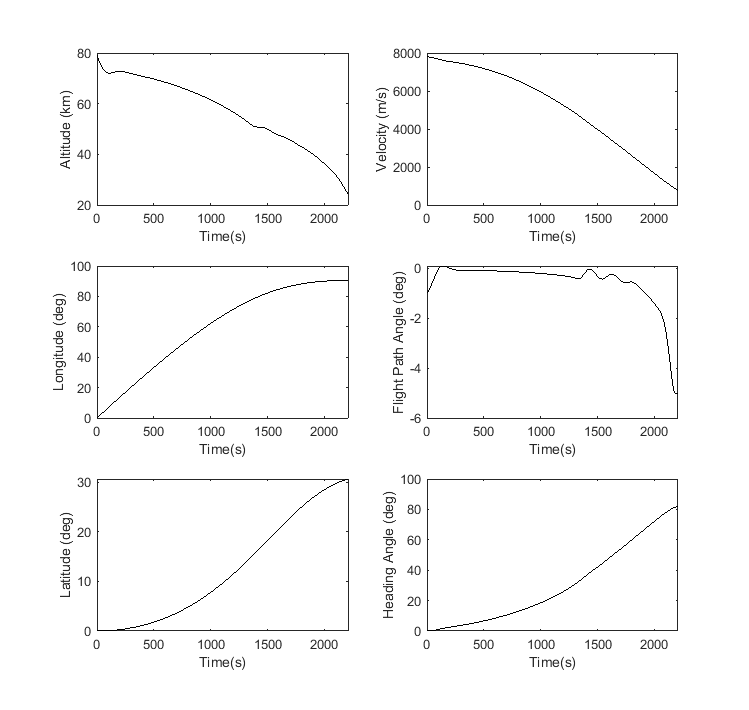
\includegraphics[width=0.7\linewidth]{figures/A1_uncertainty-analysis/SpaceShuttleq1}
\caption{}
\label{fig:SpaceShuttleq1}
\end{figure}
\begin{figure}[H]
\centering
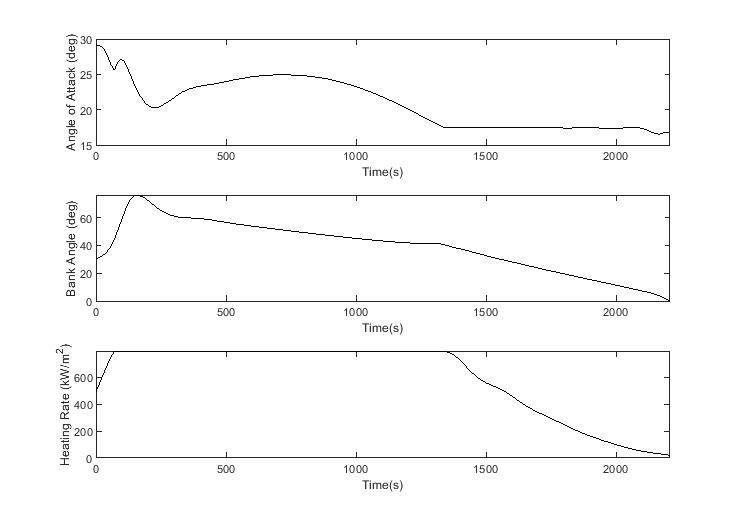
\includegraphics[width=0.7\linewidth]{figures/A1_uncertainty-analysis/SpaceShuttleq2}
\caption{}
\label{fig:SpaceShuttleq2}
\end{figure}


\section{Optimised Trajectory Verification}

\textcolor{red}{XXX Add verification here (possiblywith one of maddocks works, or a single stage to orbit, or space shuttle)}
\textcolor{red}{XXX  this is the section that descibes the error in 'timestep' as requested by reviewer, though there are multiple other factors. 'A Comparison of Accuracy and Computational E ciency of Three Pseudospectral Methods' also uses matlabs ODE45 for error comparison}.

\section{Optimised Trajectory Analysis}

This section presents an example of the convergence and verification of a trajectory optimised using GPOPS-2, within LODESTAR. The convergence and verification of a maximum payload-to-orbit trajectory solution, with SPARTAN fly-back (Case 11) is shown. 

\subsection{Mesh History}

\begin{figure}[ht]
	\centering
	\includegraphics[width=0.8\linewidth]{../LODESTAR_FINAL/Results/mode11/MeshHistory}
	\caption{The mesh history of each phase of the optimised, maximum payload-to-orbit trajectory with SPARTAN fly-back (Case 11). the phases are shown in each subfigure as follows: a) first stage rocket, b) SPARTAN acceleration, c) SPARTAN fly-back and d) third stage.}
	\label{fig:MeshHistory}
\end{figure}
The mesh history of the optimal trajectory solution is shown in Figure \ref{fig:MeshHistory}. The mesh is updated by GPOPS-2 in each iteration of the optimal solution. It can be observed that the meshes of the first and third stage rockets contain significantly less node points at the final iteration than the meshes of the SPARTAN's acceleration and return. This is due to the relatively simple dynamics and shorter flight time of the first and third stages. The first stage shows a cluster of nodes at the beginning of its trajectory, in the subsonic, transonic and low Mach regimes. In this region, the aerodynamics are changing rapidly, and the nodes are clustered to accurately capture the dynamic behaviour of the vehicle. After transition occurs to supersonic flight, the aerodynamics and engine performance of the vehicle change more slowly, and the nodes become more widely spaced. In contrast, the acceleration of the SPARTAN shows significant node density throughout. The operation of the SPARTAN is complex, as the dynamics of the vehicle and the performance of the scramjet engines vary significantly, even during relatively level flight. For this reason, the nodes of the return flight show even greater density. The trajectory conditions change significantly as the SPARTAN performs skipping manoeuvres, and transitions through the various return phases, necessitating high node density to capture the vehicle dynamics, particularly between powered and unpowered flight. The trajectories of the SPARTAN also last for a significantly longer time than the rocket trajectories, requiring more total nodes to accurately capture the vehicle dynamics. The third stage shows the least nodes at the final mesh iteration, as the dynamics of the third stage are relatively simple. Some node  clustering is observed in the first part of the trajectory, where the atmospheric density is still significant. 



\subsection{Verification}

After a trajectory has been calculated, it must be verified to ensure that the optimal control solver has converged correctly. Details on this verification are provided in Section \ref{sec:verification}. Figure \ref{fig:HamiltonianStandard} shows the Hamiltonian time history for the optimised trajectory solution of Case 11. For an optimal solution to be found, the Hamiltonian should be equal to 0 at all points over every phase. In a practical solution, a Hamiltonian close to 0 is acceptable, which is observable over all phases in the optimised solution. The Hamiltonian is close to 0 at all points of the trajectory, indicating that an optimal solution has been found. 
\begin{figure}[ht]
	\centering
	\includegraphics[width=0.9\linewidth]{../LODESTAR_FINAL/Results/mode11/HamiltonianStandard}
	\caption{The Hamiltonian time history of each phase of the maximum payload-to-orbit optimised trajectory, with SPARTAN fly-back (Case 11).}
	\label{fig:HamiltonianStandard}
\end{figure}

The next step in the verification process is to ensure that the dynamic constraints of the optimal control problem holds across the entire solution, ie. $\dot{\textbf{x}}(t) = f[t,\textbf{x}(t),\textbf{u}(t)]$. This is the most important step in the verification process, which checks that the optimal control solver has converged correctly, so that the physical dynamics of the vehicle are being correctly represented by the polynomial approximations within GPOPS-2. The dynamic constraints are tested by first calculating the dynamics of each vehicle at every node of the solution, using the vehicle simulations. These dynamics are then integrated over time using trapezoidal integration, starting at the initial conditions of each phase. The integrated dynamics are then compared to the states of the optimised solution. If the dynamic constraints have been satisfied, then the integrated dynamics of the system will be equal to the state variables of the solution. The error in the dynamic constraints of each state are shown in Figure \ref{fig:VerificationStandard}, calculated as the difference between the integrated dynamics and each state variable, normalised to the range of the state variable. 
It can be observed that all errors in the dynamic constraints are very small. The error that is present is likely to be due to the inaccuracies of the trapezoidal method, which is significantly less accurate than the approximating polynomials of the pseudospectral method. 



\begin{figure}[ht]
	\centering
	\includegraphics[width=0.9\linewidth]{../LODESTAR_FINAL/Results/mode11/VerificationStandard}
	\caption{The error between the integrated dynamics of the system, and the solution states of each phase of the maximum payload-to-orbit optimised trajectory, with SPARTAN fly-back (Case 11). Normalised to the range of each state.}
	\label{fig:VerificationStandard}
\end{figure}

The final verification step is a forward simulation of each phase. This forward simulation compares the solution state with a simulation which is forward integrated using only the controls of each stage. This is the most stringent method of checking the validity of the solution dynamics. However, it is expected that this verification will have significantly higher errors than the check which verifies the dynamics of each state independently, as the interdependencies of each state come into play, and small errors are compounded. Figure \ref{fig:ForwardErrorStandard} shows the error between the forward simulation and the solution states. As described in Section \ref{sec:verification}, the forward simulation of the return flight is separated into three segments, at 1/6th and 1/3rd of the flight time. The errors in the forward simulation of each stage are observed to be acceptably small, significantly under 1\% in all cases, and it is evident that compounding errors are the cause of the most extreme deviations. 

\begin{figure}[ht]
	\centering
	\includegraphics[width=0.9\linewidth]{../LODESTAR_FINAL/Results/mode11/ForwardErrorStandard}
	\caption{The error between the forward simulated states, and the solution states of each phase of the maximum payload-to-orbit optimised trajectory, with SPARTAN fly-back (Case 11). Normalised to the range of each state.}
	\label{fig:ForwardErrorStandard}
\end{figure}



\chapter{Modelling and Simulation}\label{Appendix:sim}
\section{Propulsion Interpolation Scheme}

\begin{figure}[ht]
	\centering
	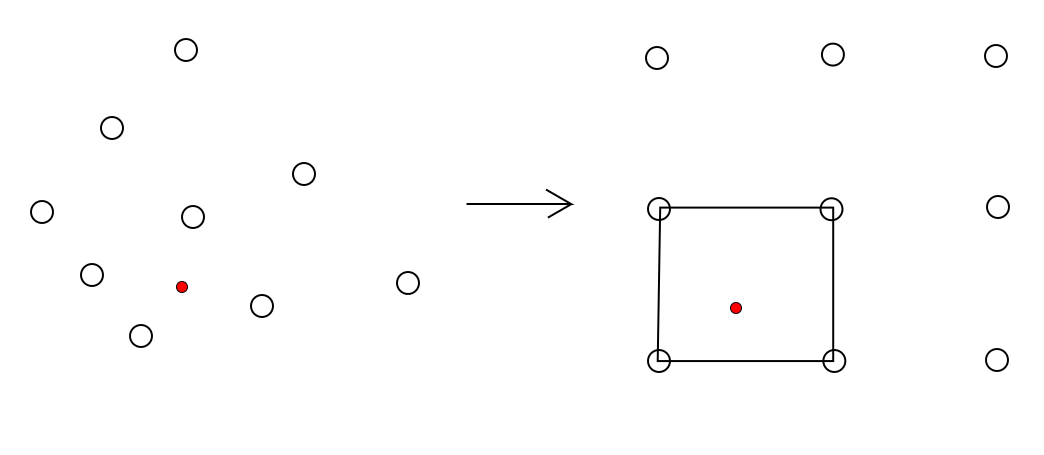
\includegraphics[width=0.8\linewidth]{figures/A1_uncertainty-analysis/interp}
	\caption{The transformation to a normalised interpolation scheme.}
	\label{fig:interp}
\end{figure}
This section describes the interpolation scheme used for the C-RESTM10 database to determine specific impulse.
The C-RESTM10 engine database consists of a set of engine conditions, including specific impulse, ordered by the inlet Mach number and temperature. This data set must be interpolated, to calculate the performance of the engine at each flight condition. However, no inlet Mach number and temperature values are repeated between any of the C-RESTM10 data points. This makes for a scattered data set which complicates the process of interpolating for specific impulse. It was observed that when interpolating for specific impulse, a scattered interpolation produces particularly poor results, and that fitting splines to the data set is the only way to produce an appropriate interpolation scheme. However, even when splines were fit, and the general trends of the specific impulse were matched, minuscule oscillations were still present in the interpolated values. These oscillations do not significantly affect a forward simulation, however, when using the vehicle model as part of an optimal control calculation, they can affect the convergence process. Consequently, it was necessary to craft a bespoke interpolation scheme in order to accurately interpolate the specific impulse of the vehicle. 

This interpolation begins by designating a new coordinate system, normalised to [0 1], running from data point with the lowest inlet temperature [0,0], to the data point with the highest inlet temperature [1,1]. Each data point is then given a set of normalised coordinates, and a cubic spline is fit to this set of normalised points using MATLAB's \textsf{griddedInterpolant} function. The normalised, orderd, data set ensures that this cubic spline is smooth, with no oscillations present. In order to interpolate at a specific location, each data point bounding the interpolation region is set as the corner of a square of data points in normalised coordinates. This is illustrated in Figure \ref{fig:interp}. The distance to each of these bounding data points is calculated, and the location to be interpolated is assigned a set of normalised coordinates. This set of normalised coordinates is used to interpolate for specific impulse. 

This process is accurate, but computationally time consuming, and would increase the computation time of the optimisation process significantly if implemented directly within the vehicle model.
 In order to expedite the interpolation process, interpolations are performed for the specific impulse for every combination of inlet Mach number and temperature present in the C-RESM10 database. This creates a grid of interpolated data points, which includes all of the data points present in the C-RESTM10 database. This grid of interpolated specific impulse values is then used as a new data set, which is now in \textsf{meshgrid} form, by which the specific impulse is interpolated. A bivariate spline is fitted to this grid of data points, using MATLAB's \textsf{griddedInterpolant} function, which is accessed by the vehicle model to determine specific impulse during flight.  







\section{SPARTAN Flow Results}
\begin{figure}[ht]
	\centering
	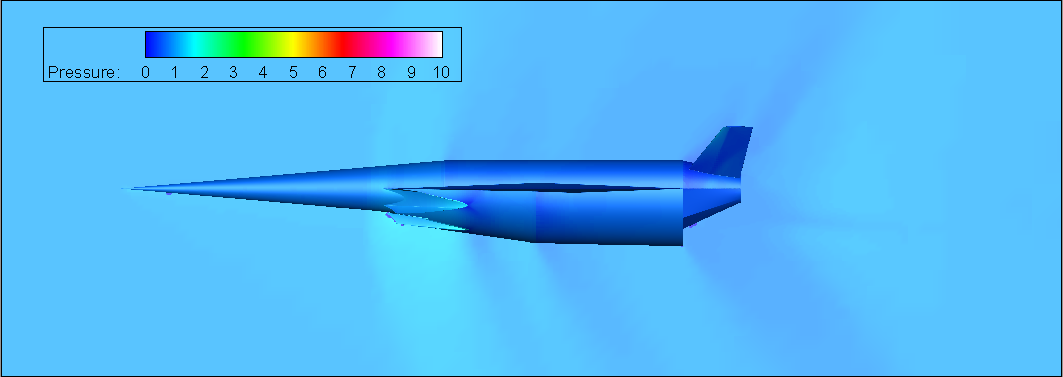
\includegraphics[width=0.9\linewidth]{figures/3_vehicle_design/M1p1AoA6}
	\caption{CART3D flow result for the SPARTAN, at Mach 1.1, 6$^\circ$ angle of attack.}
	\label{fig:M1}
\end{figure}
\begin{figure}[ht]
	\centering
	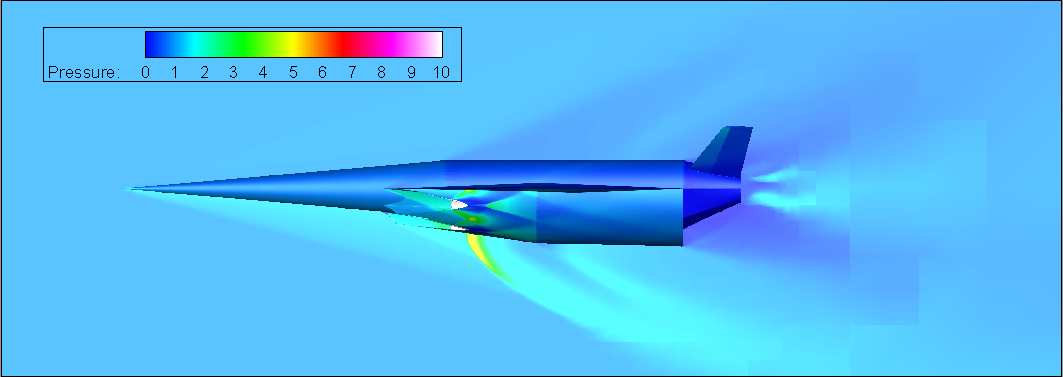
\includegraphics[width=0.9\linewidth]{figures/3_vehicle_design/M3AoA6}
	\caption{CART3D flow result for the SPARTAN, at Mach 3, 6$^\circ$ angle of attack.}
	\label{fig:M3AoA6}
\end{figure}
This section shows additional flow results for the SPARTAN, calculated using Cart3D.
Figures \ref{fig:M1} and \ref{fig:M3AoA6} show flow results for the SPARTAN, at Mach numbers of 1.1 and 3 respectively. It can be observed that at Mach 1.1, the bow shock is not significant, and the shock structure that is evident at higher speeds has not yet formed. At Mach 3, the unstarted C-REST engines are evident, causing significant amounts of the air entering the inlet to be expelled. Shock-shock interaction structures are evident on the cowl of the engines, causing areas of localised high pressure.


\FloatBarrier
\section{Cart3D Mesh}
\begin{figure}[ht]
	\centering
	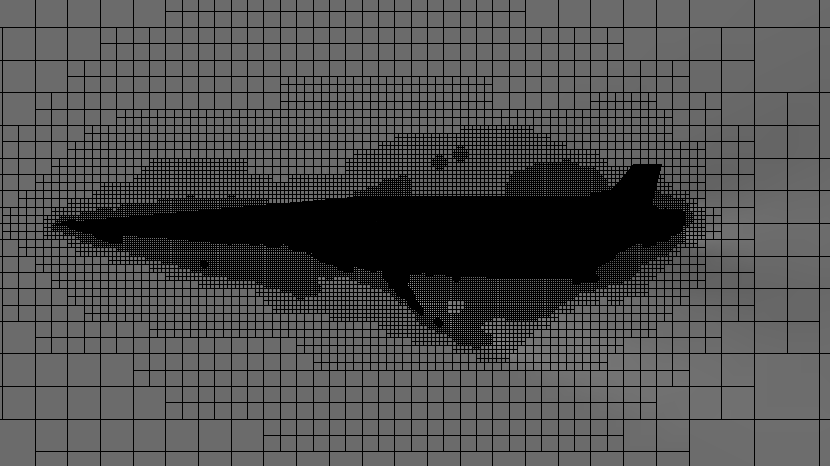
\includegraphics[width=0.7\linewidth]{figures/3_vehicle_design/M3AoA6GRID}
	\caption{Adapted mesh of the SPARTAN at Mach 6 3$^\circ$ angle of attack.}
	\label{fig:M3AoA6GRID}
\end{figure}

\begin{figure}[ht]
	\centering
	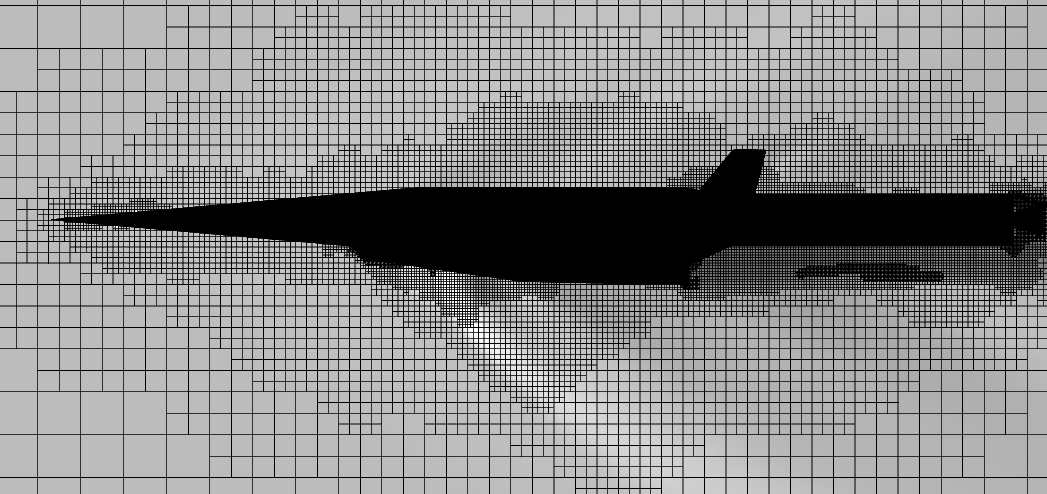
\includegraphics[width=0.7\linewidth]{figures/3_vehicle_design/CARTmesh}
	\caption{Adapted mesh around the SPARTAN and first stage vehicles, flying at Mach 2, -1$^\circ$ angle of attack.}
	\label{fig:CARTmesh}
\end{figure}
This section illustrates the converged meshes used by Cart3D.
Figures \ref{fig:M3AoA6GRID} and \ref{fig:CARTmesh} show adapted meshes for Cart3D solutions of the SPARTAN, and the SPARTAN and first stage. These meshes have been generated adaptively by Cart3D during the solution process. It can be observed that the mesh clusters around the vehicle, particularly in regions where strong shocks are present, where the mesh clusters at the shock front. 



\FloatBarrier
\section{Performance of the SPARTAN During Fly-Back}
Figure \ref{fig:returnIspStandard} shows the performance of the SPARTAN during the boost phase, described in Section \ref{sec:boost}. 

\begin{figure}[ht]
	\centering
	\includegraphics[width=0.7\linewidth]{../LODESTAR_FINAL/Results/mode11/returnIspStandard}
	\caption{The performance of the SPARTAN during the boost phase. Light blue indicates that the scramjet engines are turned on.}
	\label{fig:returnIspStandard}
\end{figure}


		\chapter{Alternate Trajectory Cases}
		\section{Trajectory With Decreased Third Stage TPS Mass}
		\textcolor{red}{XXX Add here as a design variation for reviewer}
		
		\section{Trajectory With Variation in Return Drag}
		I should maybe do a variation of just the return drag - "the performance of the launch system may be significantly different on the ascent and return trajectories (in addition to the engine flowpaths)"
		
		\section{Maximum Payload-To-Orbit Trajectory With Dynamic Pressure Constraint}\label{sec:Appendix_qconst}
		\textcolor{red}{XXX update this, make sure to update values too, used in ascent section}
		The maximum payload-to-orbit trajectory of the launch system with no SPARTAN fly-back (Case 2) was found to involve a significant altitude raising manoeuvre in the middle of the acceleration trajectory of the SPARTAN. Discerning the benefits of this altitude raising manoeuvre proved complex, requiring a trajectory to be calculated in which the altitude raising manoeuvre is prevented from occurring. This section describes an optimised trajectory in which the middle section of the SPARTAN's acceleration is constrained to flight at maximum dynamic pressure. 
		
		 This trajectory was optimised for maximum payload-to-orbit, with a 50kPa dynamic constraint between Mach numbers of 6 and 8, the region in which the altitude raising manoeuvre was observed to occur. This constraint successfully removed the altitude raising manoeuvre from the maximum payload-to-orbit optimised trajectory, allowing for a comparison to be made to quantify the benefits of the altitude raising manoeuvre. This comparison is made in Section \ref{sec:optimisednoreturn}. Figures \ref{fig:FirstStageqConstrained68},  \ref{fig:SecondStageqConstrained68} and \ref{fig:ThirdStageqConstrained68} show the maximum payload-to-orbit trajectory constrained to 50kPa between Mach numbers 6 to 8, and Table \ref{tab:constrained68} details key parameters of the trajectory. 
		
	\begin{table}[ht]
	\centering
\begin{tabular}{l c } 
	\hline \textbf{Trajectory Condition}
	& Value

	\\
	\hline \textbf{Payload to Orbit (kg)}
	& \textbf{\PayloadToOrbitqconstrainedNoReturn}
	\\
	\textbf{Total $\eta_{exergy}$ (\%)}
	& \textbf{\totalExergyEffqconstrainedNoReturn}
	\\
	\hline 
	\textbf{1$^{st}$ Stage $\eta_{exergy}$ (\%)}
	& \textbf{\firstExergyEffqconstrainedNoReturn}
	\\
	\textbf{Separation Alt, 1$\rightarrow$2 (km)}
	& \firstsecondSeparationAltqconstrainedNoReturn
	\\
	\textbf{Separation v, 1$\rightarrow$2 (m/s)}
	& \firstsecondSeparationvqconstrainedNoReturn
	\\
	\textbf{Separation $\gamma$, 1$\rightarrow$2 (deg)}
	& \firstsecondSeparationgammaqconstrainedNoReturn
	\\
	\hline 
	\textbf{2$^{nd}$ Stage $\eta_{exergy}$ (\%)}
	& \textbf{\secondExergyEffqconstrainedNoReturn}
	\\
	\textbf{Separation Alt, 2$\rightarrow$3 (km)}
	& \secondthirdSeparationAltqconstrainedNoReturn
	\\
	\textbf{Separation $v$, 2$\rightarrow$3 (m/s)}
	& \secondthirdSeparationvqconstrainedNoReturn
	\\
	\textbf{Separation $\gamma$, 2$\rightarrow$3 (deg)}
	& \secondthirdSeparationgammaqconstrainedNoReturn
	\\
	\textbf{2$^{nd}$ Stage Flight Time (s)}
	& \secondFlightTimeqconstrainedNoReturn
	\\
	\textbf{2$^{nd}$ Stage Distance Flown (km)}
	& \SecondDistqconstrainedNoReturn
	\\
	\hline 
	\textbf{3$^{rd}$ Stage $\eta_{exergy}$ (\%)}
	& \textbf{\thirddExergyEffqconstrainedNoReturn}
	\\
	\textbf{3$^{rd}$ Stage $t$, $q >$ 5kpa (s)}
	& \thirdqOverFiveqconstrainedNoReturn
	\\
	\textbf{3$^{rd}$ Stage max $\alpha$ (deg)}
	& \thirdmaxAoAqconstrainedNoReturn
	\\
	\textbf{3$^{rd}$ Stage Fuel Mass (kg)}
	& \thirdmFuelqconstrainedNoReturn
	\\
	\hline 
\end{tabular} 
\caption{A summary of key results from the maximum payload-to-orbit trajectory, constrained to 50kPa between Mach numbers 6 to 8.}
\label{tab:constrained68}

	\end{table}
		
\begin{figure}[th]
\centering
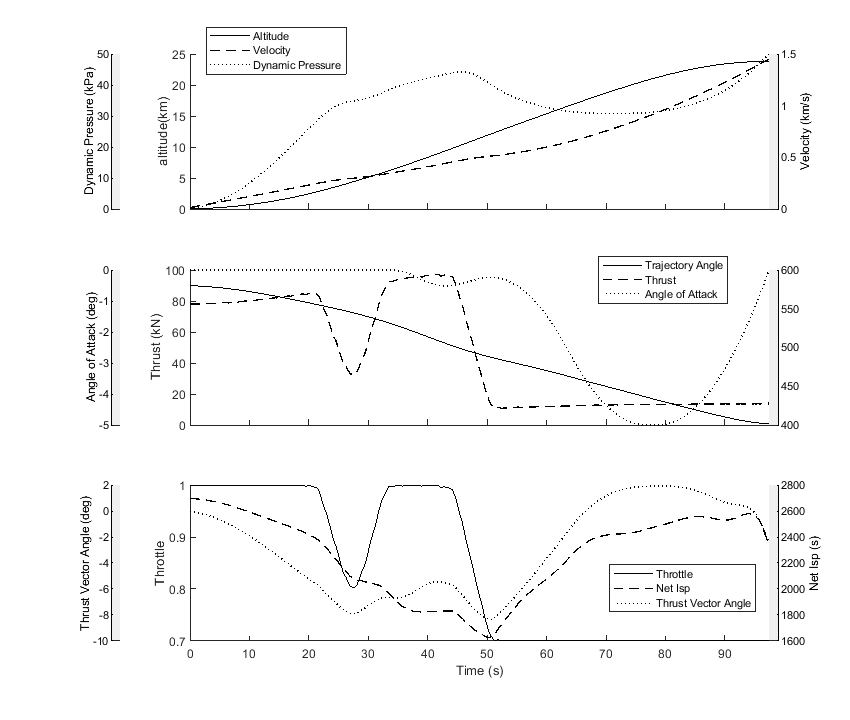
\includegraphics[width=0.9\linewidth]{../LODESTAR_FINAL/Results/10-qconstrained/FirstStageConstq}
\caption{The optimised maximum payload-to-orbit trajectory of the launch system constrained to 50kPa between Mach numbers 6 to 8, under power of the first stage rocket.}
\label{fig:FirstStageqConstrained68}
\end{figure}
		
\begin{figure}[th]
\centering
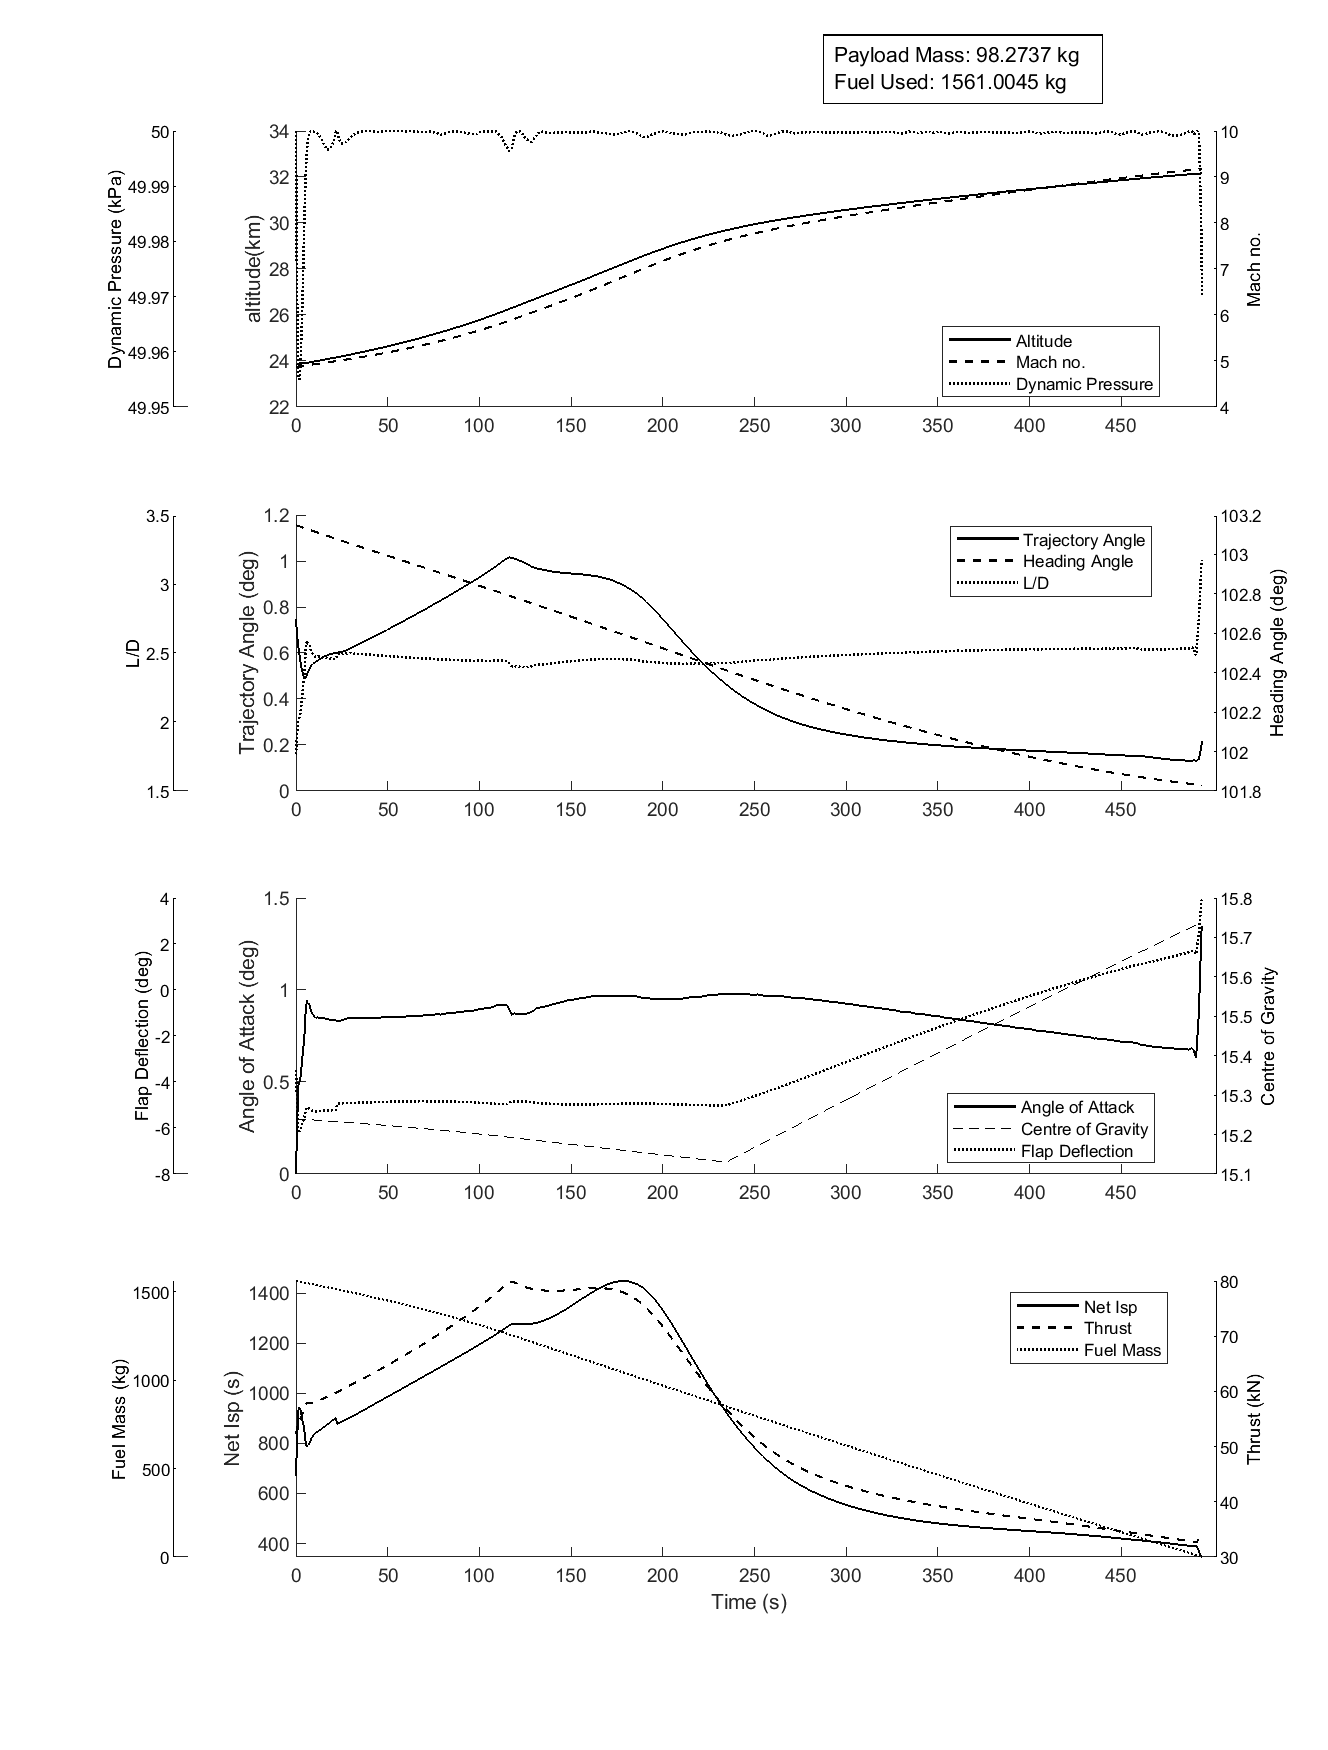
\includegraphics[width=0.9\linewidth]{../LODESTAR_FINAL/Results/10-qconstrained/SecondStageConstq}
\caption{The optimised maximum payload-to-orbit trajectory of the SPARTAN, constrained to 50kPa between Mach numbers 6 to 8.}
\label{fig:SecondStageqConstrained68}
\end{figure}

\begin{figure}[th]
\centering
\includegraphics[width=0.9\linewidth]{../LODESTAR_FINAL/Results/10-qconstrained/ThirdStageConstq}
\caption{The third stage trajectory of the launch system flying the maximum payload-to-orbit trajectory, constrained to 50kPa between Mach numbers 6 to 8.}
\label{fig:ThirdStageqConstrained68}
\end{figure}










\section{Sonic Boom Ground Effects}
\begin{figure}[ht]
	\centering
	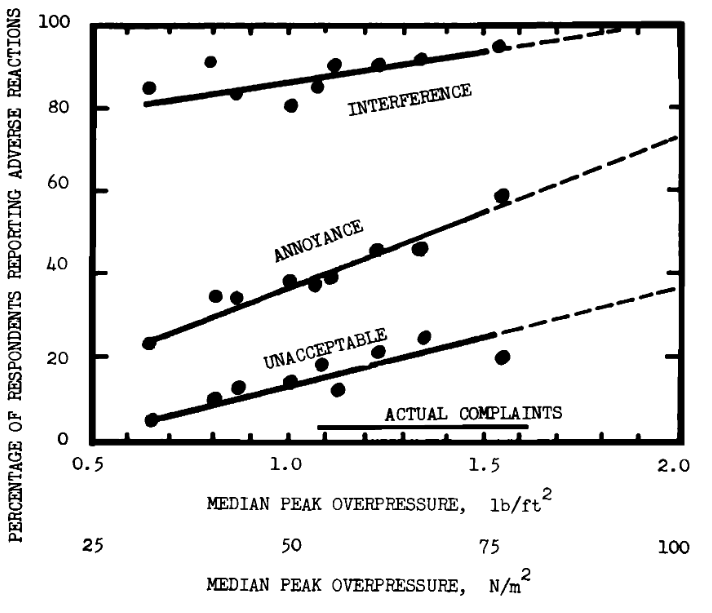
\includegraphics[width=0.6\linewidth]{figures/6_FlyBack/OverPressureResponse}
	\caption{The level of population annoyance with increasing overpressure.}
	\label{fig:OverPressureResponse}
\end{figure}

The flight of a hypersonic vehicle has the potential to create significant overpressures on the ground due to sonic booms. This section describes the effects of the sonic booms generated by the SPARTAN. 

Even when a hypersonic vehicle is flying at high altitudes, the overpressures on the ground may still be large enough to have detrimental effects on any populated areas being overflown. The overpressure from sonic booms can cause significant annoyance to the populace, or in more extreme cases, long term damage to building structures or peoples health. 
When the SPARTAN is launched to a sun synchronous orbit from the Equatorial Launch Australia launch site, it flies over a significant portion of Papua. Fortunately, Papua is sparsely populated, and the number of towns flown over by the SPARTAN will be low. However the effects on these population centres may still be significant. In order to assess the impact of the SPARTAN's flight, the magnitude of the overpressure from its sonic booms must be calculated. 
\begin{figure}[ht]
	\centering
	\includegraphics[width=0.9\linewidth]{../LODESTAR_FINAL/Results/mode11/OverPressureStandard}
	\caption{The sonic boom overpressure on the ground, for the optimised trajectory path (Case 11).}
	\label{fig:OverPressureStandard}
\end{figure}

The sonic boom overpressures are estimated using the 'first cut' estimation technique \cite{Carlson1972}. This estimation technique can approximate sonic boom overpressures moderately well, and is useful as a first approximation to the sonic boom overpressures generated by an aerospace vehicle. The overpressures generated by the SPARTAN are calculated over its trajectory, shown in Figure \ref{fig:OverPressureStandard}. It is found that overpressures of up to 375.3Pa occur during flight over land during the maximum payload-to-orbit trajectory of the SPARTAN. These overpressures have a low but significant probability of causing cosmetic damage to structures (~1.5\% for plaster and ~0.4\% for glass)\cite{Hershey1976}. In addition, overpressures of these magnitudes have been rated as unacceptably annoying to the majority populace being overflown, as shown in Figure \ref{fig:OverPressureResponse}. 
These overpressures indicate that overflight of populated areas may not be reasonable for the SPARTAN flying its maximum payload-to-orbit trajectory path, with fly-back (Case 11). 


%http://www.dtic.mil/dtic/tr/fulltext/u2/a028512.pdf





\section{Alternate Launch Location}

In this section, an alternate southerly launch is investigated for the rocket-scramjet-rocket launch system, in the case that flight over Papua is not possible. This launch occurs from Streaky Bay, the possible location of a launch site being developed by Southern Launch Australia\cite{Council2016}. The maximum payload-to-orbit has been calculated from this launch site using LODESTAR. Figure \ref{fig:GroundTrackAlternate} shows the ground track of this optimised trajectory, and Table \ref{tab:summaryalternate} details a summary of the key trajectory parameters. The shape of this optimised trajectory is very similar to the optimal trajectory of the launch system launched from the Northern Territory (Case 11). The first stage initially pitches towards the west, separating the SPARTAN in a westerly direction. The SPARTAN then performs a banking manoeuvre to the south, and a pull-up before third stage release. After separation, the SPARTAN exhibits initial turn, boost-skip and approach phases during fly-back, with the scramjet engine igniting three times at the troughs of the first three skips, in the same manner as when launching northerly. A higher payload to orbit is achieved when launching from a southerly location, attaining a total of \PayloadToOrbitAlternate kg of payload-to-orbit, an increase of +2.9\% compared to northerly launch. This payload increase is caused by the rotation of the Earth hindering, rather than assisting, when launching into a retrograde orbit, making launch from a more southerly point desirable. 


\begin{figure}[th]
	\centering
	\includegraphics[width=1\linewidth]{../LODESTAR_FINAL/Results/mode01/GroundTrackAlternate}
	\caption{The optimised maximum payload-to-orbit trajectory of the launch system launching onto a southerly orbit, from Streaky Bay.}
	\label{fig:GroundTrackAlternate}
\end{figure}

\begin{table}
	\centering
	\begin{tabular}{l c} 
		\hline \textbf{Trajectory Condition}
		& Value

		\\
		\hline \textbf{Payload to Orbit (kg)}
		& \textbf{\PayloadToOrbitAlternate}
		\\
		\textbf{Total $\eta_{exergy}$ (\%)}
		& \textbf{\totalExergyEffAlternate}
		\\
		\hline 
		\textbf{1$^{st}$ Stage $\eta_{exergy}$ (\%)}
		& \textbf{\firstExergyEffAlternate}
		\\
		\textbf{Separation Alt, 1$\rightarrow$2 (km)}
		& \firstsecondSeparationAltAlternate
		\\
		\textbf{Separation v, 1$\rightarrow$2 (m/s)}
		& \firstsecondSeparationvAlternate
		\\
		\textbf{Separation $\gamma$, 1$\rightarrow$2 (deg)}
		& \firstsecondSeparationgammaAlternate
		\\
		\hline 
		\textbf{2$^{nd}$ Stage $\eta_{exergy}$ (\%)}
		& \textbf{\secondExergyEffAlternate}
		\\
		\textbf{Separation Alt, 2$\rightarrow$3 (km)}
		& \secondthirdSeparationAltAlternate
		\\
		\textbf{Separation $v$, 2$\rightarrow$3 (m/s)}
		& \secondthirdSeparationvAlternate
		\\
		\textbf{Separation $\gamma$, 2$\rightarrow$3 (deg)}
		& \secondthirdSeparationgammaAlternate
		\\
		\textbf{2$^{nd}$ Stage Flight Time (s)}
		& \secondFlightTimeAlternate
		\\
		\textbf{2$^{nd}$ Stage Distance Flown (km)}
		& \SecondDistAlternate
		\\
		\textbf{2$^{nd}$ Stage Return Fuel (kg)}
		& \returnFuelAlternate
		\\
		\textbf{2$^{nd}$ Stage Return Distance (km)}
		& \returnDistAlternate
		\\
		\hline 
		\textbf{3$^{rd}$ Stage $\eta_{exergy}$ (\%)}
		& \textbf{\thirddExergyEffAlternate}
		\\
		\textbf{3$^{rd}$ Stage $t$, $q >$ 5kpa (s)}
		& \thirdqOverFiveAlternate
		\\
		\textbf{3$^{rd}$ Stage max $\alpha$ (deg)}
		& \thirdmaxAoAAlternate
		\\
		\textbf{3$^{rd}$ Stage Fuel Mass (kg)}
		& \thirdmFuelAlternate
		\\
		\hline 
	\end{tabular} 
	\caption{A summary of key trajectory parameters of the maximum payload-to-orbit trajectory launched in a southerly direction.}
	\label{tab:summaryalternate}
\end{table}




		
		\chapter{Trajectory Plot Comparisons}\label{sec:Appendix_trajectorycomparisons}
		
		\textcolor{red}{XXX update these}
		
This section contains trajectory plot comparisons for the sensitivity studies performed in Section \ref{sec:sensitivityNoReturn} and \ref{sec:sensitivity}. Comparisons and analyses between these trajectories are performed in the relevant sections. 
		\clearpage
		\section{Optimised Ascent Trajectory Comparisons With No Fly-Back}
		
		\subsection{Case 3: Maximum Dynamic Pressure Sensitivity Comparison}\label{sec:app_comparison20}
		
		
\begin{figure}[!ht]
\centering
\includegraphics[width=1\linewidth]{../LODESTAR_FINAL/Results/mode20/SecondStageComparison}
\caption{Comparison of SPARTAN ascent trajectories with variation in the maximum dynamic pressure of the SPARTAN.}
\label{fig:SecondStageComparison1}
\end{figure}

\begin{figure}[!th]
\centering
\includegraphics[width=1\linewidth]{../LODESTAR_FINAL/Results/mode20/ThirdStageComparison}
\caption{Comparison of third stage rocket ascent trajectories with variation in the maximum dynamic pressure of the SPARTAN.}
\label{fig:ThirdStageComparison1}
\end{figure}
\FloatBarrier

\clearpage

\subsection{Case 4: SPARTAN Drag Sensitivity Comparison}\label{sec:app_comparison40}

\begin{figure}[!th]
\centering
\includegraphics[width=1\linewidth]{../LODESTAR_FINAL/Results/mode40/SecondStageComparison}
\caption{Comparison of SPARTAN ascent trajectories with variation in the drag of the SPARTAN.}
\label{fig:SecondStageComparison3}
\end{figure}

\begin{figure}[!th]
\centering
\includegraphics[width=1\linewidth]{../LODESTAR_FINAL/Results/mode40/ThirdStageComparison}
\caption{Comparison of third stage rocket ascent trajectories with variation in the drag of the SPARTAN.}
\label{fig:ThirdStageComparison3}
\end{figure}
\FloatBarrier
\clearpage
\subsection{Case 5: SPARTAN Specific Impulse Sensitivity Comparison}\label{sec:app_comparison30}


\begin{figure}[!th]
	\centering
	\includegraphics[width=1\linewidth]{../LODESTAR_FINAL/Results/mode30/SecondStageComparison}
	\caption{Comparison of SPARTAN ascent trajectories with variation in the specific impulse of the SPARTAN.}
	\label{fig:SecondStageComparison2}
	
\end{figure}
\begin{figure}[!th]
	\centering
	\includegraphics[width=1\linewidth]{../LODESTAR_FINAL/Results/mode30/ThirdStageComparison}
	\caption{Comparison of third stage rocket ascent trajectories with variation in the specific impulse of the SPARTAN.}
	\label{fig:ThirdStageComparison2}
\end{figure}
\FloatBarrier
\clearpage
\subsection{Case 6: SPARTAN Mass Sensitivity Comparison}\label{sec:app_comparison100}

\begin{figure}[!th]
\centering
\includegraphics[width=1\linewidth]{../LODESTAR_FINAL/Results/mode100/SecondStageComparison}
\caption{Comparison of SPARTAN ascent trajectories with variation in the mass of the SPARTAN.}
\label{fig:SecondStageComparison4}
\end{figure}

\begin{figure}[!th]
\centering
\includegraphics[width=1\linewidth]{../LODESTAR_FINAL/Results/mode100/ThirdStageComparison}
\caption{Comparison of third stage rocket ascent trajectories with variation in the mass of the SPARTAN.}
\label{fig:ThirdStageComparison4}
\end{figure}
\FloatBarrier
\clearpage
\subsection{Case 7: SPARTAN Fuel Mass Sensitivity Comparison}\label{sec:app_comparison110}
\begin{figure}[!th]
\centering
\includegraphics[width=1\linewidth]{../LODESTAR_FINAL/Results/mode110/SecondStageComparison}
\caption{Comparison of SPARTAN ascent trajectories with variation in the fuel mass of the SPARTAN.}
\label{fig:SecondStageComparison5}
\end{figure}

\begin{figure}[!th]
\centering
\includegraphics[width=1\linewidth]{../LODESTAR_FINAL/Results/mode110/ThirdStageComparison}
\caption{Comparison of third stage rocket ascent trajectories with variation in the fuel mass of the SPARTAN.}
\label{fig:ThirdStageComparison5}
\end{figure}
\FloatBarrier
\clearpage
\subsection{Case 8: Third Stage Mass Sensitivity Comparison}\label{sec:app_comparison80}

\begin{figure}[!th]
\centering
\includegraphics[width=1\linewidth]{../LODESTAR_FINAL/Results/mode80/SecondStageComparison}
\caption{Comparison of SPARTAN ascent trajectories with variation in the mass of the third stage.}
\label{fig:SecondStageComparison6}
\end{figure}


\begin{figure}[!th]
\centering
\includegraphics[width=1\linewidth]{../LODESTAR_FINAL/Results/mode80/ThirdStageComparison}
\caption{Comparison of third stage rocket ascent trajectories with variation in the mass of the third stage.}
\label{fig:ThirdStageComparison6}
\end{figure}

\FloatBarrier
\clearpage
\subsection{Case 9: Third Stage Specific Impulse Sensitivity Comparison}\label{sec:app_comparison90}

\begin{figure}[!th]
	\centering
	\includegraphics[width=1\linewidth]{../LODESTAR_FINAL/Results/mode90/SecondStageComparison}
	\caption{Comparison of SPARTAN ascent trajectories with variation in the specific impulse of the third stage.}
	\label{fig:SecondStageComparison7}
\end{figure}

\begin{figure}[!th]
\centering
\includegraphics[width=1\linewidth]{../LODESTAR_FINAL/Results/mode90/ThirdStageComparison}
\caption{Comparison of third stage rocket ascent trajectories with variation in the specific impulse of the third stage.}
\label{fig:ThirdStageComparison7}
\end{figure}
\FloatBarrier
\clearpage
\subsection{Case 10:Third Stage Drag Sensitivity Comparison}\label{sec:app_comparison70}

\begin{figure}[!th]
\centering
\includegraphics[width=1\linewidth]{../LODESTAR_FINAL/Results/mode70/SecondStageComparison}
\caption{Comparison of SPARTAN ascent trajectories with variation in the drag of the third stage.}
\label{fig:SecondStageComparison8}
\end{figure}


\begin{figure}[!th]
\centering
\includegraphics[width=1\linewidth]{../LODESTAR_FINAL/Results/mode70/ThirdStageComparison}
\caption{Comparison of third stage rocket ascent trajectories with variation in the drag of the third stage.}
\label{fig:ThirdStageComparison8}
\end{figure}

\FloatBarrier
\clearpage
\section{Optimised Ascent Trajectory Comparisons With Fly-Back}
\FloatBarrier
\subsection{Case 12: Dynamic Pressure Sensitivity Comparison}\label{sec:app_comparison21}
\begin{figure}[!th]
\centering
\includegraphics[width=1\linewidth]{../LODESTAR_FINAL/Results/mode21/SecondStageComparison}
\caption{Comparison of SPARTAN ascent trajectories with variation in the maximum dynamic pressure of the SPARTAN.}
\label{fig:SecondStageComparison9}
\end{figure}

\begin{figure}[!th]
\centering
\includegraphics[width=1\linewidth]{../LODESTAR_FINAL/Results/mode21/ThirdStageComparison}
\caption{Comparison of third stage rocket ascent trajectories with variation in the maximum dynamic pressure of the SPARTAN.}
\label{fig:ThirdStageComparison9}
\end{figure}

\begin{figure}[!th]
\centering
\includegraphics[width=1\linewidth]{../LODESTAR_FINAL/Results/mode21/ReturnComparison}
\caption{Comparison of SPARTAN return trajectories with variation in the maximum dynamic pressure of the SPARTAN.}
\label{fig:ReturnComparison}
\end{figure}



\FloatBarrier
\clearpage
\subsection{Case 13: SPARTAN Drag Sensitivity Comparison}\label{sec:app_comparison41}
\begin{figure}[!th]
\centering
\includegraphics[width=1\linewidth]{../LODESTAR_FINAL/Results/mode41/SecondStageComparison}
\caption{Comparison of SPARTAN ascent trajectories with variation in the drag of the SPARTAN.}
\label{fig:SecondStageComparison11}
\end{figure}

\begin{figure}[!th]
\centering
\includegraphics[width=1\linewidth]{../LODESTAR_FINAL/Results/mode41/ThirdStageComparison}
\caption{Comparison of third stage rocket ascent trajectories with variation in the drag of the SPARTAN.}
\label{fig:ThirdStageComparison11}
\end{figure}

\begin{figure}[!th]
\centering
\includegraphics[width=1\linewidth]{../LODESTAR_FINAL/Results/mode41/ReturnComparison}
\caption{Comparison of SPARTAN return trajectories with variation in the drag of the SPARTAN.}
\label{fig:ReturnComparison11}
\end{figure}

\FloatBarrier
\clearpage
\subsection{Case 14:SPARTAN Specific Impulse Sensitivity Comparison}\label{sec:app_comparison31}
\begin{figure}[!th]
	\centering
	\includegraphics[width=1\linewidth]{../LODESTAR_FINAL/Results/mode31/SecondStageComparison}
	\caption{Comparison of SPARTAN ascent trajectories with variation in the specific impulse of the SPARTAN.}
	\label{fig:SecondStageComparison10}
\end{figure}

\begin{figure}[!th]
	\centering
	\includegraphics[width=1\linewidth]{../LODESTAR_FINAL/Results/mode31/ThirdStageComparison}
	\caption{Comparison of third stage rocket ascent trajectories with variation in the specific impulse of the SPARTAN.}
	\label{fig:ThirdStageComparison10}
\end{figure}

\begin{figure}[!th]
	\centering
	\includegraphics[width=1\linewidth]{../LODESTAR_FINAL/Results/mode31/ReturnComparison}
	\caption{Comparison of SPARTAN return trajectories with variation in the specific impulse of the SPARTAN.}
	\label{fig:ReturnComparison10}
\end{figure}
\FloatBarrier
\clearpage
\subsection{Case 15: SPARTAN Mass Sensitivity Comparison}\label{sec:app_comparison101}

\begin{figure}[!th]
\centering
\includegraphics[width=1\linewidth]{../LODESTAR_FINAL/Results/mode101/SecondStageComparison}
\caption{Comparison of SPARTAN ascent trajectories with variation in the mass of the SPARTAN.}
\label{fig:SecondStageComparison12}
\end{figure}

\begin{figure}[!th]
\centering
\includegraphics[width=1\linewidth]{../LODESTAR_FINAL/Results/mode101/ThirdStageComparison}
\caption{Comparison of third stage rocket ascent trajectories with variation in the mass of the SPARTAN.}
\label{fig:ThirdStageComparison12}
\end{figure}

\begin{figure}[!th]
\centering
\includegraphics[width=1\linewidth]{../LODESTAR_FINAL/Results/mode101/ReturnComparison}
\caption{Comparison of SPARTAN return trajectories with variation in the mass of the SPARTAN.}
\label{fig:ReturnComparison12}
\end{figure}

\FloatBarrier
\clearpage
\subsection{Case 16: SPARTAN Fuel Mass Sensitivity Comparison}\label{sec:app_comparison111}

\begin{figure}[!th]
\centering
\includegraphics[width=1\linewidth]{../LODESTAR_FINAL/Results/mode111/SecondStageComparison}
\caption{Comparison of SPARTAN ascent trajectories with variation in the fuel mass of the SPARTAN.}
\label{fig:SecondStageComparison13}
\end{figure}

\begin{figure}[!th]
\centering
\includegraphics[width=1\linewidth]{../LODESTAR_FINAL/Results/mode111/ThirdStageComparison}
\caption{Comparison of third stage rocket ascent trajectories with variation in the fuel mass of the SPARTAN.}
\label{fig:ThirdStageComparison13}
\end{figure}

\begin{figure}[!th]
\centering
\includegraphics[width=1\linewidth]{../LODESTAR_FINAL/Results/mode111/ReturnComparison}
\caption{Comparison of SPARTAN return trajectories with variation in the fuel mass of the SPARTAN.}
\label{fig:ReturnComparison13}
\end{figure}


\FloatBarrier
\clearpage
\subsection{Case 17: Third Stage Mass Sensitivity Comparison}\label{sec:app_comparison81}
\begin{figure}[!th]
\centering
\includegraphics[width=1\linewidth]{../LODESTAR_FINAL/Results/mode81/SecondStageComparison}
\caption{Comparison of SPARTAN ascent trajectories with variation in the mass of the third stage.}
\label{fig:SecondStageComparison14}
\end{figure}

\begin{figure}[!th]
\centering
\includegraphics[width=1\linewidth]{../LODESTAR_FINAL/Results/mode81/ThirdStageComparison}
\caption{Comparison of third stage rocket ascent trajectories with variation in the mass of the third stage.}
\label{fig:ThirdStageComparison14}
\end{figure}



\begin{figure}[!th]
	\centering
	\includegraphics[width=1\linewidth]{../LODESTAR_FINAL/Results/mode81/ReturnComparison}
	\caption{Comparison of SPARTAN return trajectories with variation in the mass of the third stage.}
	\label{fig:ReturnComparison14}
\end{figure}
\FloatBarrier
\clearpage
\subsection{Case 18: Third Stage Specific Impulse Sensitivity Comparison}\label{sec:app_comparison91}

\begin{figure}[!th]
\centering
\includegraphics[width=1\linewidth]{../LODESTAR_FINAL/Results/mode91/SecondStageComparison}
\caption{Comparison of SPARTAN ascent trajectories with variation in the specific impulse of the third stage.}
\label{fig:SecondStageComparison15}
\end{figure}


\begin{figure}[!th]
\centering
\includegraphics[width=1\linewidth]{../LODESTAR_FINAL/Results/mode91/ThirdStageComparison}
\caption{Comparison of third stage rocket ascent trajectories with variation in the specific impulse of the third stage.}
\label{fig:ThirdStageComparison15}
\end{figure}


\begin{figure}[!th]
\centering
\includegraphics[width=1\linewidth]{../LODESTAR_FINAL/Results/mode91/ReturnComparison}
\caption{Comparison of SPARTAN return trajectories with variation in the specific impulse of the third stage.}
\label{fig:ReturnComparison15}
\end{figure}


\chapter{Viscous Drag Variation}
\textcolor{red}{XXX Will need to redo this with variation for all stages}

This section presents the sensitivity of the launch system performance to variations in the viscous drag of the SPARTAN. This sensitivity analysis is intended as a reference, to indicate the magnitude of variations in the viscous drag of the SPARTAN due to variations in modelling methods, and is unlikely to be indicative of any physical design variations.
The viscous drag component of the SPARTAN's aerodynamics is calculated using flat plate correlations, which require an estimation of the laminar to turbulent transition point on the body of the SPARTAN\cite{Ward2018}. This transition point is difficult to estimate to a high degree of accuracy, and can have a significant effect on the viscous drag of an aircraft\cite{Ward2018}.
The viscous drag component of the SPARTAN's aerodynamics is varied, in order to assess the impact of the viscous drag model used. Optimal trajectories are calculated with the viscous drag set at levels of 20\%, 50\%, 107\% and 115\% of the baseline, which correspond to the possible viscous drag range due to transition point variation. Table \ref{tab:viscous} details key trajectory parameters of the optimised trajectories, and Figures \ref{fig:SecondStageComparison-}, \ref{fig:ThirdStageComparison-} and \ref{fig:ReturnComparison-} show comparison plots of the optimised trajectories. The sensitivity of the launch system to the viscous drag of the SPARTAN is shown to be relatively low, as the deviations in the viscous drag model are expected to be small, relative to the range tested. This low sensitivity indicating that the modelling process of the viscous drag is unlikely to have a large effect on the accuracy of the maximum payload-to-orbit solution.

\begin{table}[ht]
	\centering
	\begin{tabular}{l c c c c c c} 
		\hline \textbf{Trajectory Condition} \qquad vC$_D$:
		&20\%
		&50\%
		&100\%
		&107\%
		&115\%
		& $\Delta/\Delta$\%vC$_D$
		\\
		\hline \textbf{Payload to Orbit (kg)}
		& \textbf{\PayloadToOrbitvCdTwenty}
		& \textbf{\PayloadToOrbitvCdFifty}
		& \textbf{\PayloadToOrbitvCdStandard}
		& \textbf{\PayloadToOrbitvCdOneHundredSeven}
		& \textbf{\PayloadToOrbitvCdOneHundredFifteen}
		&\textbf{-2.5}
		\\
		\textbf{Payload Variation (\%)}
		& \PayloadVarvCdTwenty
		& \PayloadVarvCdFifty
		& \PayloadVarvCdStandard
		& \PayloadVarvCdOneHundredSeven
		& \PayloadVarvCdOneHundredFifteen
		&-0.31
		\\
		\textbf{Total $\eta_{exergy}$ (\%)}
		& \textbf{\totalExergyEffvCdTwenty}
		& \textbf{\totalExergyEffvCdFifty}
		& \textbf{\totalExergyEffvCdStandard}
		& \textbf{\totalExergyEffvCdOneHundredSeven}
		& \textbf{\totalExergyEffvCdOneHundredFifteen}
		& \textbf{-0.00024}
		\\
		\hline 
		\textbf{1$^{st}$ Stage $\eta_{exergy}$ (\%)}
		& \textbf{\firstExergyEffvCdTwenty}
		& \textbf{\firstExergyEffvCdFifty}
		& \textbf{\firstExergyEffvCdStandard}
		& \textbf{\firstExergyEffvCdOneHundredSeven}
		& \textbf{\firstExergyEffvCdOneHundredFifteen}
		& -
		\\
		\textbf{Separation Alt, 1$\rightarrow$2 (km)}
		& \firstsecondSeparationAltvCdTwenty
		& \firstsecondSeparationAltvCdFifty
		& \firstsecondSeparationAltvCdStandard
		& \firstsecondSeparationAltvCdOneHundredSeven
		& \firstsecondSeparationAltvCdOneHundredFifteen
		& -
		\\
		\textbf{Separation v, 1$\rightarrow$2 (m/s)}
		& \firstsecondSeparationvvCdTwenty
		& \firstsecondSeparationvvCdFifty
		& \firstsecondSeparationvvCdStandard
		& \firstsecondSeparationvvCdOneHundredSeven
		& \firstsecondSeparationvvCdOneHundredFifteen
		& -
		\\
		\textbf{Separation $\gamma$, 1$\rightarrow$2 (deg)}
		& \firstsecondSeparationgammavCdTwenty
		& \firstsecondSeparationgammavCdFifty
		& \firstsecondSeparationgammavCdStandard
		& \firstsecondSeparationgammavCdOneHundredSeven
		& \firstsecondSeparationgammavCdOneHundredFifteen
		& -
		\\
		\hline 
		\textbf{2$^{nd}$ Stage $\eta_{exergy}$ (\%)}
		& \textbf{\secondExergyEffvCdTwenty}
		& \textbf{\secondExergyEffvCdFifty}
		& \textbf{\secondExergyEffvCdStandard}
		& \textbf{\secondExergyEffvCdOneHundredSeven}
		& \textbf{\secondExergyEffvCdOneHundredFifteen}
		& \textbf{-0.064}
		\\
		\textbf{Separation Alt, 2$\rightarrow$3 (km)}
		& \secondthirdSeparationAltvCdTwenty
		& \secondthirdSeparationAltvCdFifty
		& \secondthirdSeparationAltvCdStandard
		& \secondthirdSeparationAltvCdOneHundredSeven
		& \secondthirdSeparationAltvCdOneHundredFifteen
		& -
		\\
		\textbf{Separation $v$, 2$\rightarrow$3 (m/s)}
		& \secondthirdSeparationvvCdTwenty
		& \secondthirdSeparationvvCdFifty
		& \secondthirdSeparationvvCdStandard
		& \secondthirdSeparationvvCdOneHundredSeven
		& \secondthirdSeparationvvCdOneHundredFifteen
		&-33.84
		\\
		\textbf{Separation $\gamma$, 2$\rightarrow$3 (deg)}
		& \secondthirdSeparationgammavCdTwenty
		& \secondthirdSeparationgammavCdFifty
		& \secondthirdSeparationgammavCdStandard
		& \secondthirdSeparationgammavCdOneHundredSeven
		& \secondthirdSeparationgammavCdOneHundredFifteen
		&-0.1
		\\
		\textbf{2$^{nd}$ Stage Flight Time (s)}
		& \secondFlightTimevCdTwenty
		& \secondFlightTimevCdFifty
		& \secondFlightTimevCdStandard
		& \secondFlightTimevCdOneHundredSeven
		& \secondFlightTimevCdOneHundredFifteen
		& -
		\\
		\textbf{2$^{nd}$ Stage Distance Flown (km)}
		& \SecondDistvCdTwenty
		& \SecondDistvCdFifty
		& \SecondDistvCdStandard
		& \SecondDistvCdOneHundredSeven
		& \SecondDistvCdOneHundredFifteen
		& -
		\\
		\textbf{2$^{nd}$ Stage Return Fuel (kg)}
		& \returnFuelvCdTwenty
		& \returnFuelvCdFifty
		& \returnFuelvCdStandard
		& \returnFuelvCdOneHundredSeven
		& \returnFuelvCdOneHundredFifteen
		& -
		\\
		\textbf{2$^{nd}$ Stage Return Distance (km)}
		& \returnDistvCdTwenty
		& \returnDistvCdFifty
		& \returnDistvCdStandard
		& \returnDistvCdOneHundredSeven
		& \returnDistvCdOneHundredFifteen
		&-21.35
		\\
		\hline 
		\textbf{3$^{rd}$ Stage $\eta_{exergy}$ (\%)}
		& \textbf{\thirddExergyEffvCdTwenty}
		& \textbf{\thirddExergyEffvCdFifty}
		& \textbf{\thirddExergyEffvCdStandard}
		& \textbf{\thirddExergyEffvCdOneHundredSeven}
		& \textbf{\thirddExergyEffvCdOneHundredFifteen}
		& \textbf{-0.249}
		\\
		\textbf{3$^{rd}$ Stage $t$, $q >$ 5kpa (s)}
		& \thirdqOverFivevCdTwenty
		& \thirdqOverFivevCdFifty
		& \thirdqOverFivevCdStandard
		& \thirdqOverFivevCdOneHundredSeven
		& \thirdqOverFivevCdOneHundredFifteen
		&-0.24
		\\
		\textbf{3$^{rd}$ Stage max $\alpha$ (deg)}
		& \thirdmaxAoAvCdTwenty
		& \thirdmaxAoAvCdFifty
		& \thirdmaxAoAvCdStandard
		& \thirdmaxAoAvCdOneHundredSeven
		& \thirdmaxAoAvCdOneHundredFifteen
		& -
		\\
		\textbf{3$^{rd}$ Stage Fuel Mass (kg)}
		& \thirdmFuelvCdTwenty
		& \thirdmFuelvCdFifty
		& \thirdmFuelvCdStandard
		& \thirdmFuelvCdOneHundredSeven
		& \thirdmFuelvCdOneHundredFifteen
		&-32.96
		\\
		\hline 
	\end{tabular} 
	\caption{Summary of key trajectory parameters with SPARTAN viscous drag variation.}
	\label{tab:viscous}
\end{table} 


\begin{figure}[!th]
\centering
\includegraphics[width=1\linewidth]{../LODESTAR_FINAL/Results/mode51/SecondStageComparison}
\caption{Comparison of SPARTAN ascent trajectories with variation in the viscous drag of the SPARTAN.}
\label{fig:SecondStageComparison-}
\end{figure}
\begin{figure}[!th]
\centering
\includegraphics[width=1\linewidth]{../LODESTAR_FINAL/Results/mode51/ThirdStageComparison}
\caption{Comparison of third stage ascent trajectories with variation in the viscous drag of the SPARTAN.}
\label{fig:ThirdStageComparison-}
\end{figure}


\begin{figure}[!th]
	\centering
	\includegraphics[width=1\linewidth]{../LODESTAR_FINAL/Results/mode51/ReturnComparison}
	\caption{Comparison of SPARTAN return trajectories with variation in the viscous drag of the SPARTAN.}
	\label{fig:ReturnComparison-}
\end{figure}
